%%%%%%%%%%%%%%%%%%%%%%%%%%%%%%%%%%%%%%%%%
% Beamer Presentation
% LaTeX Template
% Version 1.0 (10/11/12)
%
% This template has been downloaded from:
% http://www.LaTeXTemplates.com
%
% License:
% CC BY-NC-SA 3.0 (http://creativecommons.org/licenses/by-nc-sa/3.0/)
%
%%%%%%%%%%%%%%%%%%%%%%%%%%%%%%%%%%%%%%%%%

%----------------------------------------------------------------------------------------
%	PACKAGES AND THEMES
%----------------------------------------------------------------------------------------

\documentclass[10pt]{beamer}

\mode<presentation> {

% The Beamer class comes with a number of default slide themes
% which change the colors and layouts of slides. Below this is a list
% of all the themes, uncomment each in turn to see what they look like.
\usetheme{metropolis}
%\usetheme{default}
%\usetheme{AnnArbor}
%\usetheme{Antibes}
%\usetheme{Bergen}
%\usetheme{Berkeley}
%\usetheme{Berlin}
%\usetheme{Boadilla}
%\usetheme{CambridgeUS}
%\usetheme{Copenhagen}
%\usetheme{Darmstadt}
%\usetheme{Dresden}
%\usetheme{Frankfurt}
%\usetheme{Goettingen}
%\usetheme{Hannover}
%\usetheme{Ilmenau}
%\usetheme{JuanLesPins}
%\usetheme{Luebeck}
%\usetheme{Madrid}
%\usetheme{Malmoe}
%\usetheme{Marburg}
%\usetheme{Montpellier}
%\usetheme{PaloAlto}
%\usetheme{Pittsburgh}
%\usetheme{Rochester}
%\usetheme{Singapore}
%\usetheme{Szeged}
%\usetheme{Warsaw}

% As well as themes, the Beamer class has a number of color themes
% for any slide theme. Uncomment each of these in turn to see how it
% changes the colors of your current slide theme.

%\usecolortheme{albatross}
%\usecolortheme{beaver}
%\usecolortheme{beetle}
%\usecolortheme{crane}
%\usecolortheme{dolphin}
%\usecolortheme{dove}
%\usecolortheme{fly}
%\usecolortheme{lily}
%\usecolortheme{orchid}
%\usecolortheme{rose}
%\usecolortheme{seagull}
%\usecolortheme{seahorse}
%\usecolortheme{whale}
%\usecolortheme{wolverine}

\setbeamertemplate{footline} % To remove the footer line in all slides uncomment this line
%\setbeamertemplate{footline}[page number] % To replace the footer line in all slides with a simple slide count uncomment this line

\setbeamertemplate{navigation symbols}{} % To remove the navigation symbols from the bottom of all slides uncomment this line
}

\usefonttheme{professionalfonts}

\setbeamertemplate{footline}[frame number]
\usepackage{graphicx} % Allows including images
\usepackage[utf8x]{inputenc}
\usepackage[turkish]{babel}
\usepackage[T1]{fontenc}
\usepackage{physics}
\usepackage{mathtools}
\usepackage{xcolor}

\usepackage{outlines}


%----------------------------------------------------------------------------------------
%	TITLE PAGE
%----------------------------------------------------------------------------------------

\title[Kollektif Nötrino Salınımları]{\huge \textbf{KOLLEKTİF EVRİLEN NÖTRİNOLARIN ÇEŞNİ DÖNÜŞÜMÜ}\vspace{0.5cm}} % The short title appears at the bottom of every slide, the full title is only on the title page

\author{\Large{İsmail Taygun Bulmuş}\vspace{1cm}} % Your name
\institute[MSGSÜ, Fizik Bölümü] % Your institution as it will appear on the bottom of every slide, may be shorthand to save space
{\vspace{1cm}
{\large \textbf{Doktora Tez Savunması}}} 


\date{06 Temmuz 2022} % Date, can be changed to a custom date

\begin{document}
\shorthandoff{=}

\begin{frame}[plain, noframenumbering]
\titlepage % Print the title page as the first slide
\end{frame}

\begin{frame}
    \frametitle{İçerik}
    \begin{outline}
        \1[\textbullet] Giriş
        \1[\textbullet] Nötrino Salınım Kinematiği
        \1[\textbullet] Salınım Hamiltonyen'i ve Madde Etkileşimleri
        \2[\textendash] MSW Resonance
        \1[\textbullet] $H_{\nu}+ H_{M}+ H_{EM}$
        \2[\textendash] SFP Resonance
        \1[\textbullet] Analitik öngörüler
        \1[\textbullet] Simülasyonlar
        \1[\textbullet] Çekirdek Sentezlenmesi
    \end{outline}
\end{frame}

\begin{frame}
    \frametitle{Giriş - İçerik}
    %\textbf{Çeşni Salınımları} 
    \begin{outline}
        \1[\textbullet] Nötrino çeşni salınımları ve hareket denklemleri
        \1[\textbullet] Madde içerisinde nötrino salınımları, MSW rezonansı ve madde bazının tanımlanması
        \1[\textbullet] Hem madde hem de elektromanyetik etkileşimler altında nötrino çeşni evrimi
        \2[\textendash] {\color{blue} Tedirgeme (perturbasyon) yöntemi ile çözüm elde etme}
        \2[\textendash] {\color{blue} İki çeşni indirgenmesi ve bazı profiller için tam çözüm eldesi}
        \2[\textendash] SFP Rezonansı
        \1[\textbullet] Landau-Zener geçiş olasılıkları ve adyabatiste kavramı
        \1[\textbullet] {\color{red}Stokes fazı ve çekirdek çökmeli süpernova (ÇÇSN) içerisinde faz etkileri}
        \1[\textbullet] {\color{red}İki çeşni yaklaşıklığı ve yaklaşıklığın geçerli olduğu durumlar}
        \1[\textbullet] {\color{blue}Nötrino öz-kırılımının kollektif çeşni evrimine olan katkısı}
        \1[\textbullet] {\color{cyan}Nötrinoların ÇÇSN çekirdek sentezindeki önemi}
    \end{outline}
\end{frame}

\begin{frame}
    \frametitle{Giriş - Motivasyon}
        \begin{minipage}{0.45\textwidth}
            \footnotesize
            \begin{outline}
                \1[\textbullet] 1987 Yılında Büyük Macellan Bulutu içerisinde bir adet süpernova meydana gelmiştir (SN1987A.)
                \1[\textbullet] SN1987A'dan gelen yaklaşık 20 adet antinötrino gözlemlenmiştir (Kamiokande, IMB ve Baksan.)
                \1[\textbullet] ÇÇSN'den Dünya'ya gelen nötrinolar ÇÇSN dinamiği hakkında bilgi taşır.
                \1[\textbullet] ÇÇSN'nin merkezinde oluşan manyetik alan ile nötrinolar etkileşir ve çeşni evrimine katkıda bulunur.
                \1[\textbullet] Nötrino çeşni salınımlarında rezonanslar meydana gelir.
            \end{outline}
            \normalsize
        \end{minipage}
        \hfill
        \begin{minipage}{0.45\textwidth}
            \begin{figure}[hbt!]
                \centering
                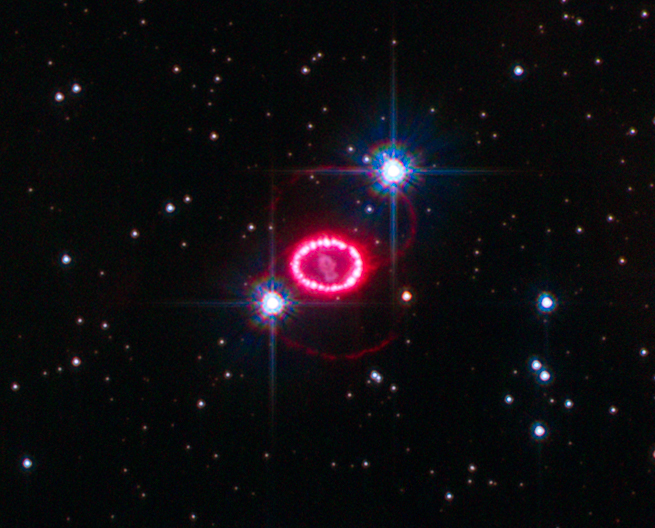
\includegraphics[width=.4\textwidth]{fig/SN1987A.jpg}
                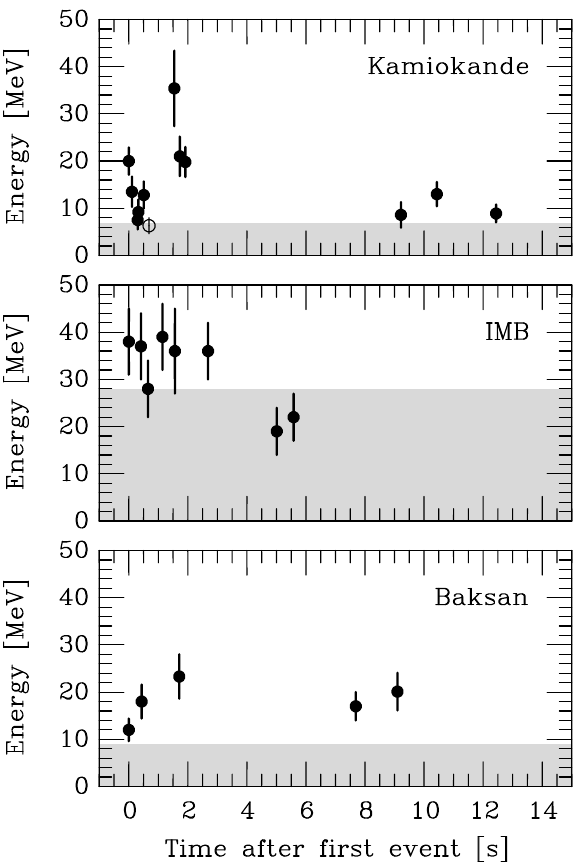
\includegraphics[width=.7\textwidth]{fig/SN1987A_neutrino.png}
                {\tiny Raffelt, 1996}
            \end{figure}
            
        \end{minipage}
\end{frame}

\begin{frame}
    \frametitle{Nötrino Salınım Kinematiği}
\begin{minipage}{0.45\textwidth}
Schrödinger tipi denklem

\begin{align*}
    i\dv{r} \ket{\Psi(r)}= H^{\text{f}}(r) \ket{\Psi(r)}
\end{align*}
Matris formunda 
\begin{equation*}
    i\dv{r} \mqty(\ket{\nu_{e}(r)} \\ \ket{\nu_{\mu}(r)}\\ \ket{\nu_{\overline{e}}(r)}\\ \ket{\nu_{\overline{\mu}}(r)}) = H^{\text{f}}(r) \mqty(\ket{\nu_{e}(r)} \\ \ket{\nu_{x}(r)}\\ \ket{\nu_{\overline{e}}(r)}\\ \ket{\nu_{\overline{x}}(r)})
\end{equation*}
\end{minipage}%
\hfill
\begin{minipage}{0.45\textwidth}
    \color{lightgray}Yoğunluk operatörü notasyonu
\begin{equation*}
    \hat{\rho} (r) = \sum_{i} a_{i} \dyad{\Psi_{i}(r)}{\Psi_{i}(r)}
\end{equation*}
Liouville - von Neumann denklemi
\begin{equation*}
    i \dv{r} \hat{\rho} = \comm{\hat{H}}{\hat{\rho}}
\end{equation*}
\end{minipage}
\end{frame}

\begin{frame}[noframenumbering]
    \frametitle{Nötrino Salınım Kinematiği}
\begin{minipage}{0.45\textwidth}
Schrödinger tipi denklem

\begin{align*}
    i\dv{r} \ket{\Psi(r)}= H^{\text{f}}(r) \ket{\Psi(r)}
\end{align*}
Matris formunda 
\begin{equation*}
    i\dv{r} \mqty(\ket{\nu_{e}(r)} \\ \ket{\nu_{\mu}(r)}\\ \ket{\nu_{\overline{e}}(r)}\\ \ket{\nu_{\overline{\mu}}(r)}) = H^{\text{f}}(r) \mqty(\ket{\nu_{e}(r)} \\ \ket{\nu_{x}(r)}\\ \ket{\nu_{\overline{e}}(r)}\\ \ket{\nu_{\overline{x}}(r)})
\end{equation*}
\end{minipage}%
\hfill
\begin{minipage}{0.45\textwidth}
    Yoğunluk operatörü notasyonu
\begin{equation*}
    \hat{\rho} (r) = \sum_{i} a_{i} \dyad{\Psi_{i}(r)}{\Psi_{i}(r)}
\end{equation*}
Liouville - von Neumann denklemi
\begin{equation*}
    i \dv{r} \hat{\rho} = \comm{\hat{H}}{\hat{\rho}}
\end{equation*}
\end{minipage}
\end{frame}

\begin{frame}
    \frametitle{Salınım Hamiltonyen'i ve Madde Etkileşimleri}
(Anti)Nötrino boşluk Hamiltonyen'i
\begin{align*}
    \hat{H}_{\nu} & = \sum^{4}_{i=1} \frac{m_{i}^{2}}{2E} \dyad{\nu_{i}}{\nu_{i}}\\
	              & = \sum_{\alpha,\beta = e,x,\bar{e},\bar{x}} \qty(\sum_{i=1,2,3,4} \frac{m_{i}^{2}}{2E} U_{\alpha i} U_{\beta i})\dyad{\nu_{\alpha}}{\nu_{\beta}}
\end{align*}
Çeşni karışım matrisi
\begin{equation*}
    U= \mqty( \cos \theta & \sin \theta & 0 & 0 \\ -\sin \theta & \cos \theta & 0 & 0 \\ 0 & 0 & \cos \theta & \sin \theta\\ 0 & 0 & - \sin \theta & \cos \theta)
\end{equation*}
\end{frame}

\begin{frame}
    \frametitle{Salınım Hamiltonyen'i ve Madde Etkileşimleri}
    \begin{outline}
        \1[\textbullet] Majorana Nötrinoları (Sıfır CP fazı)
        \1[\textbullet] İki çeşni, $ \nu_{e}, \nu_{x} $ ($2$ nötrino $, 2 $ antinötrino)
        \1[\textbullet] Atmosferik kütle kare farkı, $ \delta m^{2}= 2.56 \time 10^{-15} $ MeV$ ^{2} $
        \1[\textbullet] Karışım açısı, $ \theta=8^{\circ}  $
        \1[\textbullet] Normal veya ters hiyerarşi
    \end{outline}
    \begin{figure}[hbt!]
        \centering
        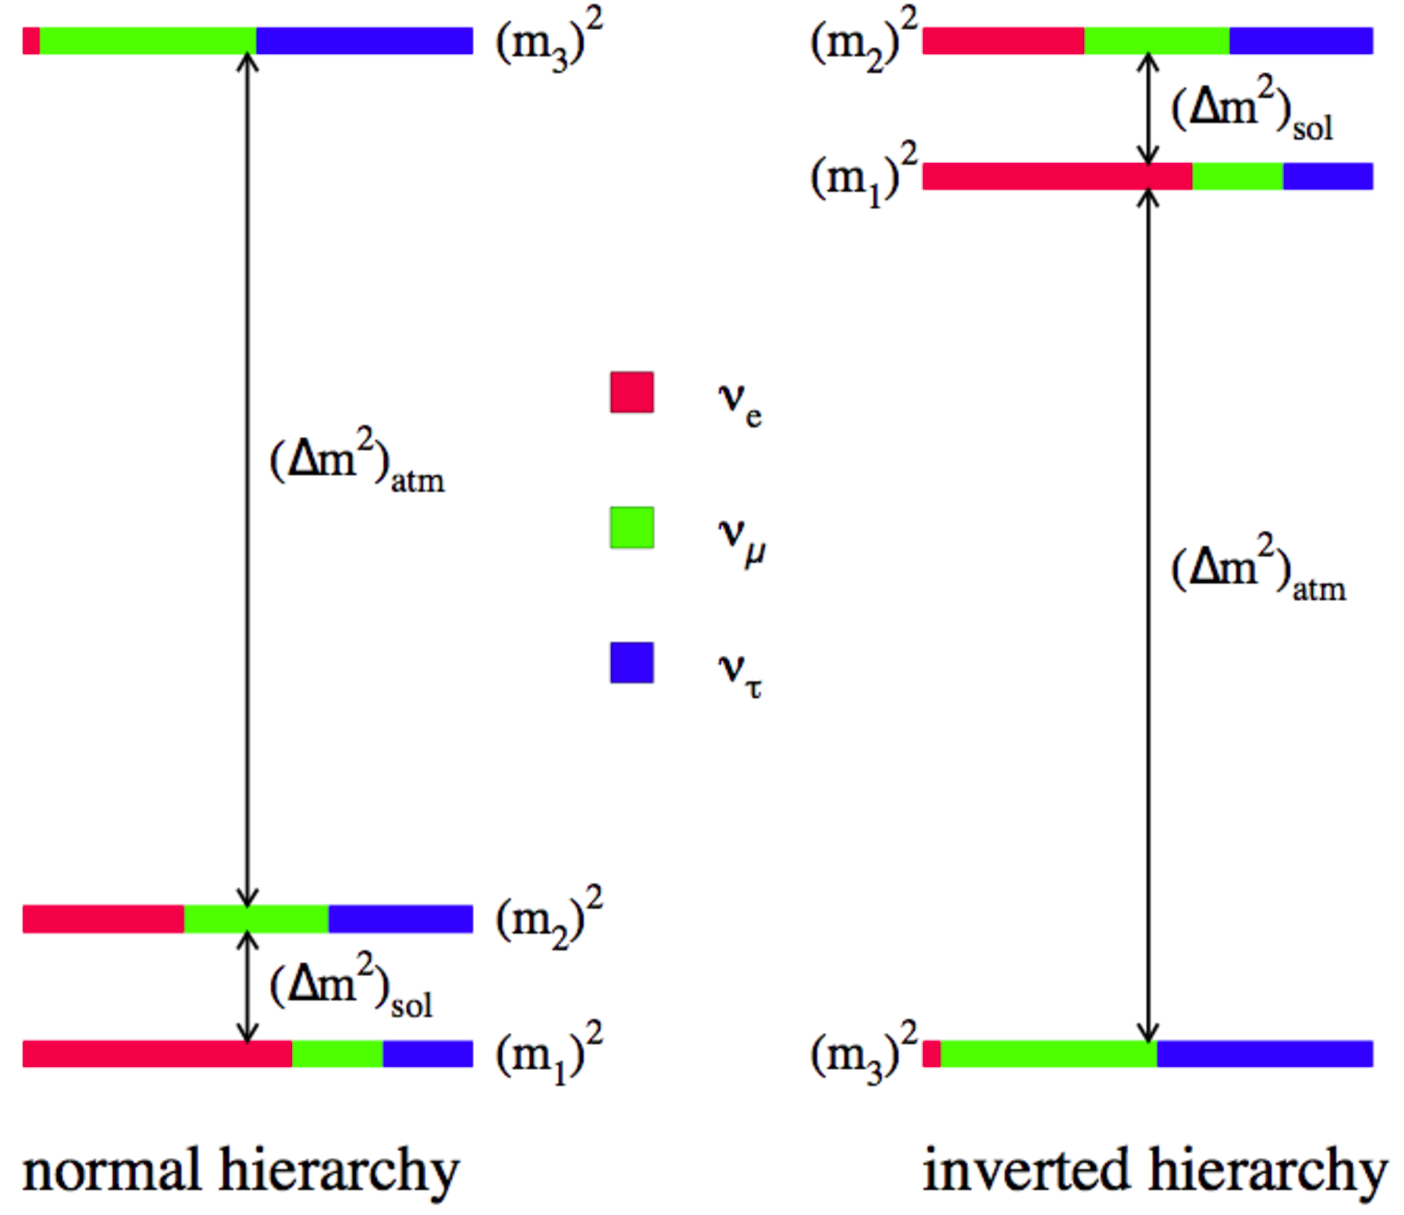
\includegraphics[width=.45\textwidth]{fig/nuHier.pdf}
    \end{figure}
\end{frame}
\begin{frame}
    \frametitle{Salınım Hamiltonyen'i ve Madde Etkileşimleri}
    Boşluk ve madde etkileşim Hamiltonyen'i
    \tiny
    \begin{align*}
        (H^{f}_{\nu,M})_{\alpha\beta} =\mqty(-\Delta c_{ 2\theta}+V_{CC}+V_{NC} & \Delta s_{ 2\theta} & 0 & 0\\ \Delta s_{ 2\theta} & \Delta c_{ 2\theta}+V_{NC} & 0 & 0 \\0 & 0 & -\Delta c_{ 2\theta}-V_{CC}-V_{NC} & \Delta s_{ 2\theta}\\ 0 & 0 & \Delta s_{ 2\theta} & \Delta c_{ 2\theta}-V_{NC} )
    \end{align*}
    \normalsize
    
    Etkileşimler
    \begin{figure}[hbt!]
        \centering
        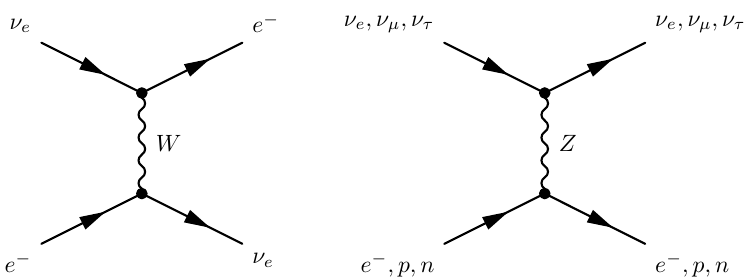
\includegraphics[width=.65\textwidth]{fig/matFeynDiag.png}
        {\tiny [Giunti, 2007]}
    \end{figure}
    \begin{align*}
        V_{CC}(r) = \sqrt{2}G_{F}N_{e}(r) \qquad& V_{NC}(r) = -\frac{\sqrt{2}}{2}G_{F}N_{n}(r)\\
        V_{CC}(r) = \sqrt{2}G_{F}n_{b}(r)Y_{e} \qquad& V_{NC}(r) = -\frac{\sqrt{2}}{2}G_{F}n_{b}(r)(1-Y_{e})
    \end{align*}
\end{frame}

\begin{frame}
    \frametitle{Salınım Hamiltonyen'i ve Madde Etkileşimleri}
    \hrulefill
    \tiny
    \begin{align*}
        (H^{f}_{\nu,M})_{\alpha\beta} =\mqty(-\Delta c_{ 2\theta}+V_{CC}+V_{NC} & \Delta s_{ 2\theta} & 0 & 0\\ \Delta s_{ 2\theta} & \Delta c_{ 2\theta}+V_{NC} & 0 & 0 \\0 & 0 & -\Delta c_{ 2\theta}-V_{CC}-V_{NC} & \Delta s_{ 2\theta}\\ 0 & 0 & \Delta s_{ 2\theta} & \Delta c_{ 2\theta}-V_{NC} )
    \end{align*}
    \normalsize
    \hrulefill

    \begin{minipage}{0.45\textwidth}
    Özdeğerler
    \tiny
    \begin{align*}
        \omega_{1} = {-M + V_{NC}+ V_{CC}/2} \\
        \omega_{2} = {+M + V_{NC}+ V_{CC}/2} \\
        \omega_{3} = {-\overline{M} - V_{NC}- V_{CC}/2}\\
        \omega_{4} = {-\overline{M} - V_{NC}- V_{CC}/2}
    \end{align*}
    \normalsize
    Burada

    {\tiny $ M, \overline{M} = \sqrt{(\Delta s_{ 2\theta})^{2}+(\Delta c_{2\theta} \pm V_{CC}/2 ) } $}.

    \end{minipage}
    \hfill
    \begin{minipage}{0.45\textwidth}
        Madde bazında hareket denklemleri
        \tiny
        \begin{equation*}
            i \dv{r} \mqty(\ket{\nu^{M}_{1}}\\ \ket{\nu^{M}_{2}}) = \mqty(\omega_{1} & -i \dv{r}\theta_{M} \\ i \dv{r}\theta_{M} & \omega_{2}) \mqty(\ket{\nu^{M}_{1}}\\ \ket{\nu^{M}_{2}})
        \end{equation*}
        \begin{equation*}
	        i \dv{r} \mqty(\ket{\nu^{M}_{3}}\\ \ket{\nu^{M}_{4}}) = \mqty(\omega_{3} & -i \dv{r}\overline{\theta}_{M} \\ i \dv{r}\overline{\theta}_{M} & \omega_{4}) \mqty(\ket{\nu^{M}_{3}}\\ \ket{\nu^{M}_{4}})
        \end{equation*}
        \normalsize
        Efektif madde karışım açısı
        \begin{equation*}
            \tan 2\theta_{M}(r) = \frac{\tan 2\theta}{1\pm \frac{V_{CC}(r)}{2\Delta c_{2\theta}}}
        \end{equation*}
    \end{minipage}
\end{frame}

\begin{frame}
    \frametitle{MSW Rezonansı}
    \hrulefill
    \tiny
    \begin{equation*}
        i \dv{r} \mqty(\ket{\nu^{M}_{1}}\\ \ket{\nu^{M}_{2}}) = \mqty(\omega_{1} & -i \dv{r}\theta_{M} \\ i \dv{r}\theta_{M} & \omega_{2}) \mqty(\ket{\nu^{M}_{1}}\\ \ket{\nu^{M}_{2}})
    \end{equation*}
    \begin{equation*}
        i \dv{r} \mqty(\ket{\nu^{M}_{3}}\\ \ket{\nu^{M}_{4}}) = \mqty(\omega_{3} & -i \dv{r}\overline{\theta}_{M} \\ i \dv{r}\overline{\theta}_{M} & \omega_{4}) \mqty(\ket{\nu^{M}_{3}}\\ \ket{\nu^{M}_{4}})
    \end{equation*}
    \normalsize
    \hrulefill
    
    \begin{minipage}{0.45\textwidth}
        \begin{figure}[hbt!]
            \centering
            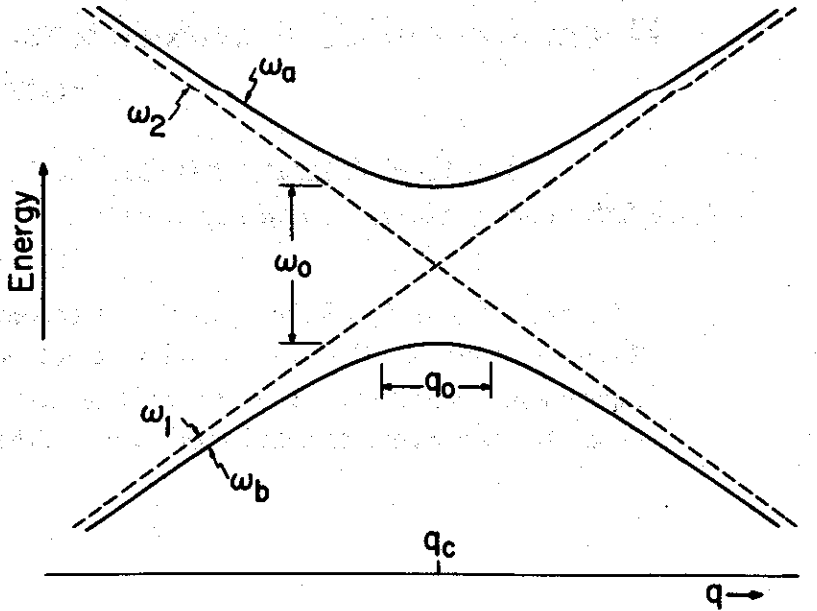
\includegraphics[width=.9\textwidth]{fig/Avoid_Crossing_With_Paramters.png}
            {\tiny [Rubbmark, 1981]}
        \end{figure}
    \end{minipage}
    \hfill
    \begin{minipage}{0.45\textwidth}
        \begin{figure}[hbt!]
            \centering
            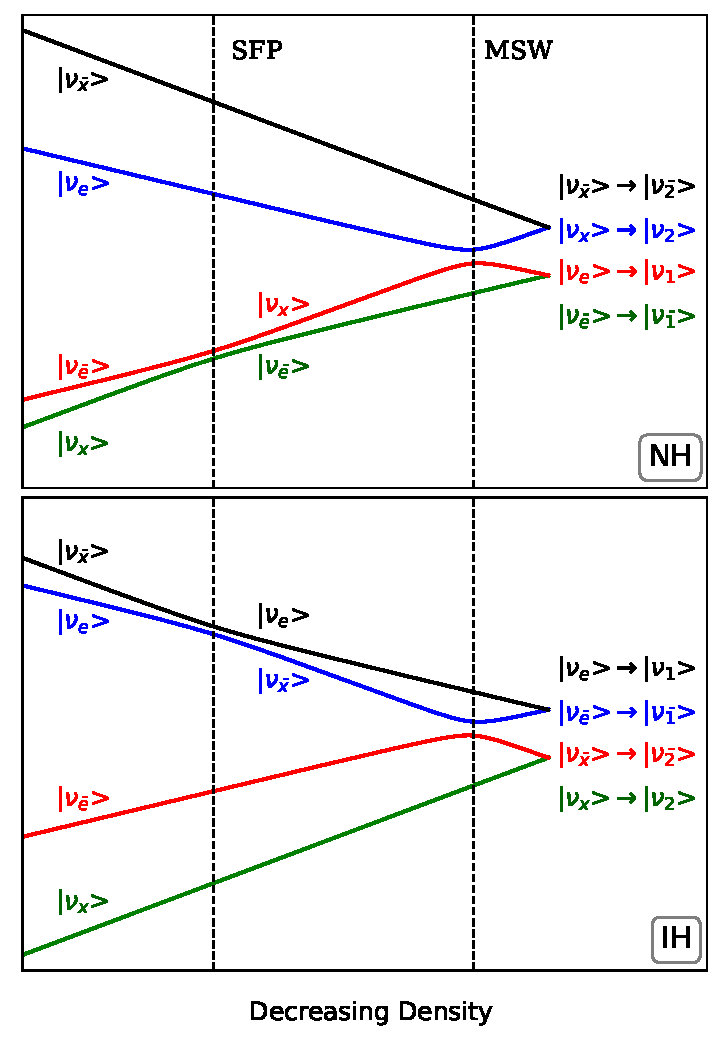
\includegraphics[width=.9\textwidth]{fig/eigenvalues.pdf}
        \end{figure}
    \end{minipage}
\end{frame}

\begin{frame}
    \frametitle{$H_{\nu}+ H_{M}+ H_{EM}$}
    Çeşni tabanında toplam Hamiltonyen matrisi
    \tiny
    \begin{equation*}
        (H_{T})_{\alpha\beta}(r) = \mqty(-\Delta c_{2\theta}+V_{CC}+V_{NC} & \Delta s_{2\theta} & 0 & \mu B\\\Delta s_{2\theta} & \Delta c_{2\theta} + V_{NC}& -\mu B & 0
        \\0 & -\mu B& -\Delta c_{2\theta}-V_{CC}-V_{NC} & \Delta s_{2\theta}\\ \mu B& 0 & \Delta s_{2\theta} & \Delta c_{2\theta}-V_{NC} )
    \end{equation*}
    \normalsize
    Madde tabanında ise
    \tiny
    \begin{align*}
        H^{M}_{T}(r) =& H^{M}_{\nu,M} + U^{\dagger}_{M} H^{f}_{EM} U_{M}\\
        =& \mqty(\omega_{1} & 0 & 0 & 0\\0 & \omega_{2} & 0 & 0\\0 & 0 & \omega_{3} & 0\\0 & 0 & 0 & \omega_{4}) + \mqty(c_{\gamma} & -s_{\gamma} & 0 & 0\\s_{\gamma} & c_{\gamma} & 0 & 0\\0 & 0 & c_{\gamma} & s_{\gamma}\\0 & 0 & s_{\gamma} & c_{\gamma})\mqty(0&0&0&\mu B\\0&0&-\mu B&0\\0&-\mu B&0&0\\\mu B&0&0&0)
    \end{align*}
    \normalsize
    Burada $ \gamma = \theta_{M} - \overline{\theta}_{M} $.
\end{frame}

\begin{frame}
    \frametitle{$H_{\nu}+ H_{M}+ H_{EM}$ - Tedirgeme}
    \begin{minipage}{0.45\textwidth}
        Baz geçiş diyagramı
        \begin{figure}[hbt!]
            \centering
            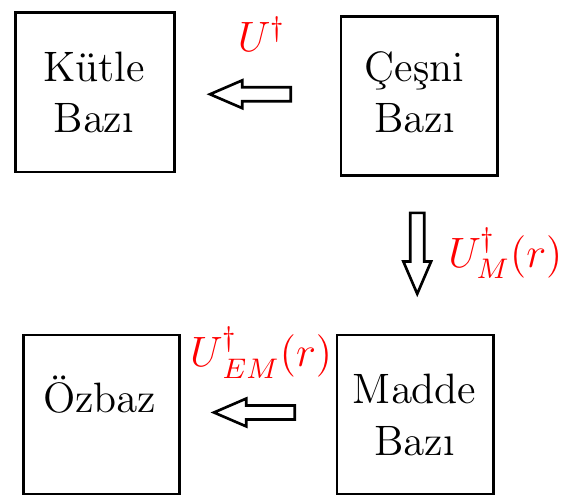
\includegraphics[width=.9\textwidth]{fig/tedirgemeDiagram.png}
        \end{figure}
        Tedirgeme yönteminin geçerli olduğu koşul.
        \begin{equation*}
            \abs{c_{\gamma}~\mu B}, \abs{s_{\gamma}~\mu B}  \ll \abs{\omega_{i}-\omega_{j}}
        \end{equation*}
    \end{minipage}
    \hfill
    \begin{minipage}{0.45\textwidth}
        \color{lightgray}
        Özdurumlar
        \tiny
        \begin{equation*}
            \mqty(
                \frac{1}{N_{1}}\ket{\nu^{EM}_{1}}\\
                \frac{1}{N_{2}}\ket{\nu^{EM}_{2}}\\
                \frac{1}{N_{3}}\ket{\nu^{EM}_{3}}\\
                \frac{1}{N_{4}}\ket{\nu^{EM}_{4}}) =
            \mqty(
                \ket{\nu^{M}_{1}}\\
                \ket{\nu^{M}_{2}}\\
                \ket{\nu^{M}_{3}}\\
                \ket{\nu^{M}_{4}})
            + \mu B s_{\gamma} \mqty(
                    \ket{\nu^{M}_{3}}/\delta \omega_{13} \\
                    \ket{\nu^{M}_{4}}/\delta \omega_{24} \\
                    \ket{\nu^{M}_{1}}/\delta \omega_{31} \\
                    \ket{\nu^{M}_{2}}/\delta \omega_{42})
        \end{equation*}
            \begin{equation*}
            \hspace{1.5cm}+ \mu B c_{\gamma} \mqty(
            \ket{\nu^{M}_{4}}/\delta \omega_{14} \\
            \ket{\nu^{M}_{3}}/\delta \omega_{23} \\
            \ket{\nu^{M}_{2}}/\delta \omega_{32} \\
            \ket{\nu^{M}_{1}}/\delta \omega_{41})
        \end{equation*}
        \begin{equation*}
            + (\mu B)^{2} \frac{\sin 2\gamma}{2} \mqty(\frac{\delta \omega_{13} - 
            \delta \omega_{14}}{\delta \omega_{12} \delta \omega_{13} 
            \delta \omega_{14}} \ket{\nu^{M}_{2}} \\
            \frac{\delta \omega_{23} - \delta \omega_{24}}{\delta \omega_{21} 
            \delta \omega_{23} \delta \omega_{24}} \ket{\nu^{M}_{1}} \\
            \frac{\delta \omega_{32} - \delta \omega_{31}}{\delta \omega_{34} 
            \delta \omega_{31} \delta \omega_{32}} \ket{\nu^{M}_{4}} \\
            \frac{\delta \omega_{42} - \delta \omega_{41}}{\delta \omega_{43} 
            \delta \omega_{41} \delta \omega_{42}} \ket{\nu^{M}_{3}})
        \end{equation*}
        \normalsize
    \end{minipage}
\end{frame}

\begin{frame}[noframenumbering]
    \frametitle{$H_{\nu}+ H_{M}+ H_{EM}$ - Tedirgeme}
    \begin{minipage}{0.45\textwidth}
        Baz geçiş diyagramı
        \begin{figure}[hbt!]
            \centering
            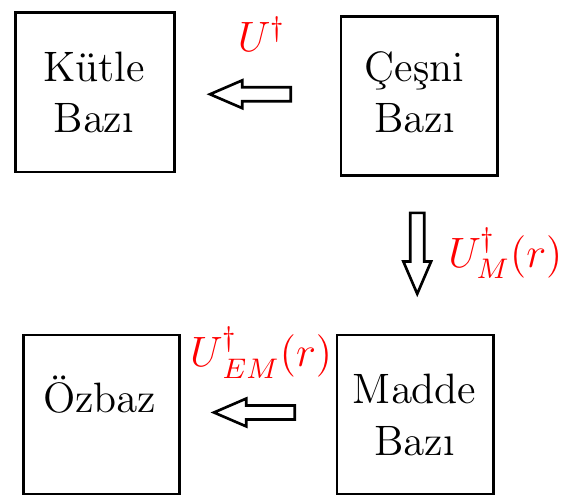
\includegraphics[width=.9\textwidth]{fig/tedirgemeDiagram.png}
        \end{figure}
        Tedirgeme yönteminin geçerli olduğu koşul.
        \begin{equation*}
            \abs{c_{\gamma}~\mu B}, \abs{s_{\gamma}~\mu B}  \ll \abs{\omega_{i}-\omega_{j}}
        \end{equation*}
    \end{minipage}
    \hfill
    \begin{minipage}{0.45\textwidth}
        Özdurumlar
        \tiny
        \begin{equation*}
            \mqty(
                \frac{1}{N_{1}}\ket{\nu^{EM}_{1}}\\
                \frac{1}{N_{2}}\ket{\nu^{EM}_{2}}\\
                \frac{1}{N_{3}}\ket{\nu^{EM}_{3}}\\
                \frac{1}{N_{4}}\ket{\nu^{EM}_{4}}) =
            \mqty(
                \ket{\nu^{M}_{1}}\\
                \ket{\nu^{M}_{2}}\\
                \ket{\nu^{M}_{3}}\\
                \ket{\nu^{M}_{4}})
            + \mu B s_{\gamma} \mqty(
                    \ket{\nu^{M}_{3}}/\delta \omega_{13} \\
                    \ket{\nu^{M}_{4}}/\delta \omega_{24} \\
                    \ket{\nu^{M}_{1}}/\delta \omega_{31} \\
                    \ket{\nu^{M}_{2}}/\delta \omega_{42})
        \end{equation*}
            \begin{equation*}
            \hspace{1.5cm}+ \mu B c_{\gamma} \mqty(
            \ket{\nu^{M}_{4}}/\delta \omega_{14} \\
            \ket{\nu^{M}_{3}}/\delta \omega_{23} \\
            \ket{\nu^{M}_{2}}/\delta \omega_{32} \\
            \ket{\nu^{M}_{1}}/\delta \omega_{41})
        \end{equation*}
        \begin{equation*}
            + (\mu B)^{2} \frac{\sin 2\gamma}{2} \mqty(\frac{\delta \omega_{13} - 
            \delta \omega_{14}}{\delta \omega_{12} \delta \omega_{13} 
            \delta \omega_{14}} \ket{\nu^{M}_{2}} \\
            \frac{\delta \omega_{23} - \delta \omega_{24}}{\delta \omega_{21} 
            \delta \omega_{23} \delta \omega_{24}} \ket{\nu^{M}_{1}} \\
            \frac{\delta \omega_{32} - \delta \omega_{31}}{\delta \omega_{34} 
            \delta \omega_{31} \delta \omega_{32}} \ket{\nu^{M}_{4}} \\
            \frac{\delta \omega_{42} - \delta \omega_{41}}{\delta \omega_{43} 
            \delta \omega_{41} \delta \omega_{42}} \ket{\nu^{M}_{3}})
        \end{equation*}
        \normalsize
    \end{minipage}
\end{frame}

\begin{frame}
    \frametitle{$H_{\nu}+ H_{M}+ H_{EM}$ - Tam Çözüm}
    Hareket denklemi
    \scriptsize
    \begin{align*}
        i\dv{}{r} \mqty(\ket{\nu_{e}} \\ \ket{\nu_{\bar{x}}}) &= 
        \mqty(0 & \mu B \\ \mu B & 2\Delta c_{2\theta}-V_{CC}-2V_{NC}    ) 
        \mqty(\ket{\nu_{e}}\\ \ket{\nu_{\bar{x}}})
    \end{align*}
    \normalsize
    İkinci dereceden diferansiyel denklem
    \scriptsize
    \begin{equation*}
        \dv[2]{\nu_{i}}{r} + \left(i\kappa_{i}+iP(r) + \frac{\dv{B}{r}}{B(r)}\right) 
    \dv{\nu_{i}}{r}+ (\mu B(r))^{2}~ \nu_{i} = 0
    \end{equation*}
    \normalsize
    {\tiny Burada $ P(r) \equiv -\sqrt{2}G_{F}(1-2Y_{e})N_{b}(r) $ ve $ \kappa_{1,2} \equiv \mp 2\Delta c_{2\theta} $}
    
    \textbf{Eksponansiyel baryon profili, sabit manyetik çözümü}
    \scriptsize
    \begin{align*}
        \nu_{i}(r) & = N_{1}^{\xi^{+}_{i}}~ _{1}F_{1}\left(\xi^{+}_{i}; 
        1+2\xi^{+}_{i}-\kappa_{i};\frac{-iP(r)}{\alpha} \right) + N_{2}^{\xi^{-}_{i}} ~ _{1}F_{1}\left(\xi^{-}_{i}; 1+2\xi^{-}_{i}-
        \kappa_{i};\frac{-iP(r)}{\alpha}\right)
    \end{align*}
    {\tiny Burada $\xi^{\mp}_{i} \equiv \frac{i(\kappa_{i} \mp \sqrt{(2\mu B)^{2} + 
    \kappa^{2}_{i} } )}{2\alpha}$ ve $ _{1}F_{1} $ Kummer fonksiyonları.}
    \normalsize
\end{frame}

\begin{frame}
    \frametitle{$H_{\nu}+ H_{M}+ H_{EM}$ - Tam Çözüm}
    Hareket denklemi
    \scriptsize
    \begin{align*}
        i\dv{}{r} \mqty(\ket{\nu_{e}} \\ \ket{\nu_{\bar{x}}}) &= 
        \mqty(0 & \mu B \\ \mu B & 2\Delta c_{2\theta}-V_{CC}-2V_{NC}    ) 
        \mqty(\ket{\nu_{e}}\\ \ket{\nu_{\bar{x}}})
    \end{align*}
    \normalsize
    İkinci dereceden diferansiyel denklem
    \scriptsize
    \begin{equation*}
        \dv[2]{\nu_{i}}{r} + \left(i\kappa_{i}+iP(r) + \frac{\dv{B}{r}}{B(r)}\right) 
    \dv{\nu_{i}}{r}+ (\mu B(r))^{2}~ \nu_{i} = 0
    \end{equation*}
    \normalsize
    {\tiny Burada $ P(r) \equiv -\sqrt{2}G_{F}(1-2Y_{e})N_{b}(r) $ ve $ \kappa_{1,2} \equiv \mp 2\Delta c_{2\theta} $}
    
    \textbf{Aynı eksponansiyel manyetik alan ve baryon profili için çözümler}
    Genelleştirilmiş hipergeometrik fonksiyonlar ve birleşmiş Laguerre polinomları.
\end{frame}

\begin{frame}
    \frametitle{$H_{\nu}+ H_{M}+ H_{EM}$ - SFP Rezonansı}
    \hrulefill
    
    \tiny
    \begin{equation*}
        (H_{T})_{\alpha\beta}(r) = \mqty(-\Delta c_{2\theta}+V_{CC}+V_{NC} & \Delta s_{2\theta} & 0 & \mu B\\\Delta s_{2\theta} & \Delta c_{2\theta} + V_{NC}& -\mu B & 0
        \\0 & -\mu B& -\Delta c_{2\theta}-V_{CC}-V_{NC} & \Delta s_{2\theta}\\ \mu B& 0 & \Delta s_{2\theta} & \Delta c_{2\theta}-V_{NC} )
    \end{equation*}
    \normalsize
    
    \hrulefill

    \begin{minipage}{0.45\textwidth}
        \footnotesize
        2 çeşniye indirgenmiş toplam Hamiltonyen
        \tiny
        \begin{equation*}
            H_{T,e\bar{x}} = \mqty(-\Delta c_{2\theta}+V_{CC}+V_{NC} & \mu B \\ \mu B & \Delta c_{2\theta}-V_{NC})
        \end{equation*}
        \begin{equation*}
	        H_{T,x\bar{e}} = \mqty(\Delta c_{2\theta}+V_{NC} & -\mu B \\ -\mu B & -\Delta c_{2\theta}-V_{CC}-V_{NC})
        \end{equation*}
        \footnotesize
        Efektif EM karışım açısı
        \begin{equation*}
            \tan 2\theta_{EM} = \frac{\mu B}{\Delta c_{2\theta} \pm V_{NC} \pm V_{CC}/2}
        \end{equation*}
        Özel elektron kesri değeri
        \begin{equation*}
            \eval{\tan 2\theta_{EM}}_{Y_{e}=0.5} = \frac{\mu B}{\Delta c_{2\theta}}
        \end{equation*}
        \normalsize
    \end{minipage}
    \hfill
    \begin{minipage}{0.45\textwidth}
        
    \end{minipage}
\end{frame}

\begin{frame}[noframenumbering]
    \frametitle{$H_{\nu}+ H_{M}+ H_{EM}$ - SFP Rezonansı}
    \hrulefill
    
    \tiny
    \begin{equation*}
        (H_{T})_{\alpha\beta}(r) = \mqty(-\Delta c_{2\theta}+V_{CC}+V_{NC} & \Delta s_{2\theta} & 0 & \mu B\\\Delta s_{2\theta} & \Delta c_{2\theta} + V_{NC}& -\mu B & 0
        \\0 & -\mu B& -\Delta c_{2\theta}-V_{CC}-V_{NC} & \Delta s_{2\theta}\\ \mu B& 0 & \Delta s_{2\theta} & \Delta c_{2\theta}-V_{NC} )
    \end{equation*}
    \normalsize
    
    \hrulefill

    \begin{minipage}{0.45\textwidth}
        \footnotesize
        2 çeşniye indirgenmiş toplam Hamiltonyen
        \tiny
        \begin{equation*}
            H_{T,e\bar{x}} = \mqty(-\Delta c_{2\theta}+V_{CC}+V_{NC} & \mu B \\ \mu B & \Delta c_{2\theta}-V_{NC})
        \end{equation*}
        \begin{equation*}
	        H_{T,x\bar{e}} = \mqty(\Delta c_{2\theta}+V_{NC} & -\mu B \\ -\mu B & -\Delta c_{2\theta}-V_{CC}-V_{NC})
        \end{equation*}
        \footnotesize
        Efektif EM karışım açısı
        \begin{equation*}
            \tan 2\theta_{EM} = \frac{\mu B}{\Delta c_{2\theta} \pm V_{NC} \pm V_{CC}/2}
        \end{equation*}
        Özel elektron kesri değeri
        \begin{equation*}
            \eval{\tan 2\theta_{EM}}_{Y_{e}=0.5} = \frac{\mu B}{\Delta c_{2\theta}}
        \end{equation*}
        \normalsize
    \end{minipage}
    \hfill
    \begin{minipage}{0.45\textwidth}
        \begin{figure}[hbt!]
            \centering
            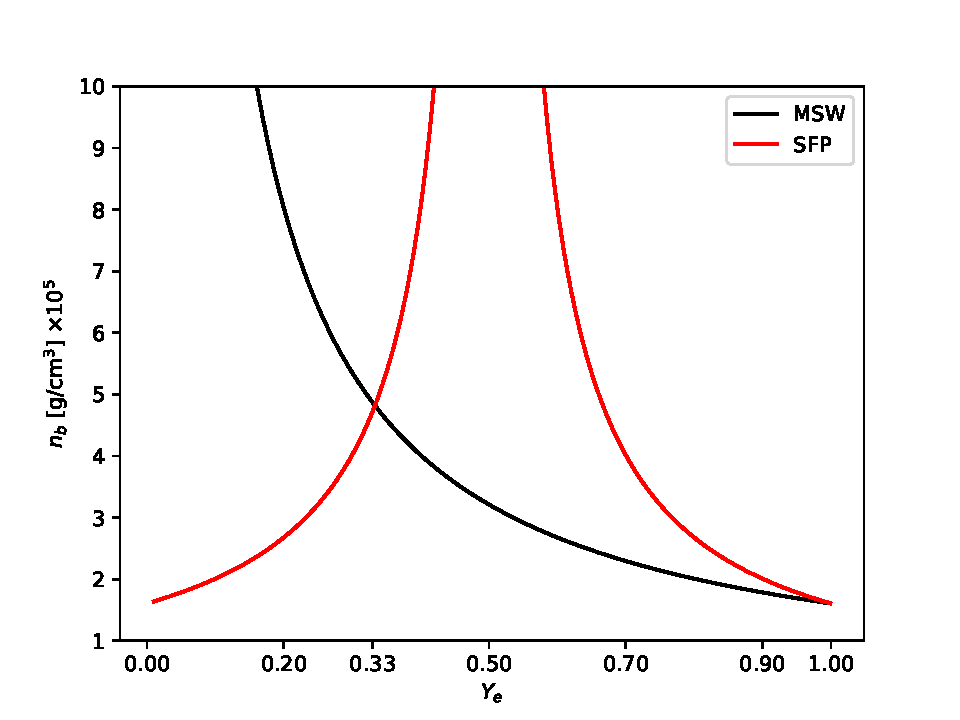
\includegraphics[width=1.2\textwidth]{fig/resonance_nb_Ye.pdf}
        \end{figure}
    \end{minipage}
\end{frame}

\begin{frame}
    \frametitle{$H_{\nu}+ H_{M}+ H_{EM}$ - Rezonanslar}
    \begin{figure}[hbt!]
        \centering
        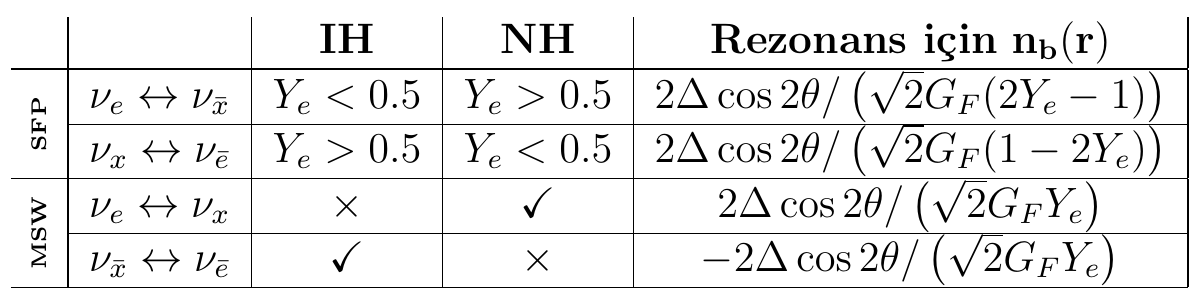
\includegraphics[width=\textwidth]{fig/rezonanslar.png}
    \end{figure}
\end{frame}

\begin{frame}
    \frametitle{$H_{\nu}+ H_{M}+ H_{EM}$ - Rezonanslar}
    Landau - Zener geçiş olasılığı, adyabatisiteye bağlıdır. Şartlar:
    \scriptsize
    \begin{enumerate}
        \item Hamiltonyen'in geçişten sorumlu olan elemanı konumdan bağımsız olmalıdır.
        \item Başlangıçtaki anlık (instantaneous) özdurumlar, başlangıç durumu ile aynı olmalıdır.
        \item Özdeğerlerin yakınlaştığı yani geçiş bölgesinde özdeğer farkları doğrusal olmalıdır.
    \end{enumerate}
    \normalsize

    \hrulefill

    \begin{minipage}{0.45\textwidth}
    \begin{figure}[hbt!]
        \centering
        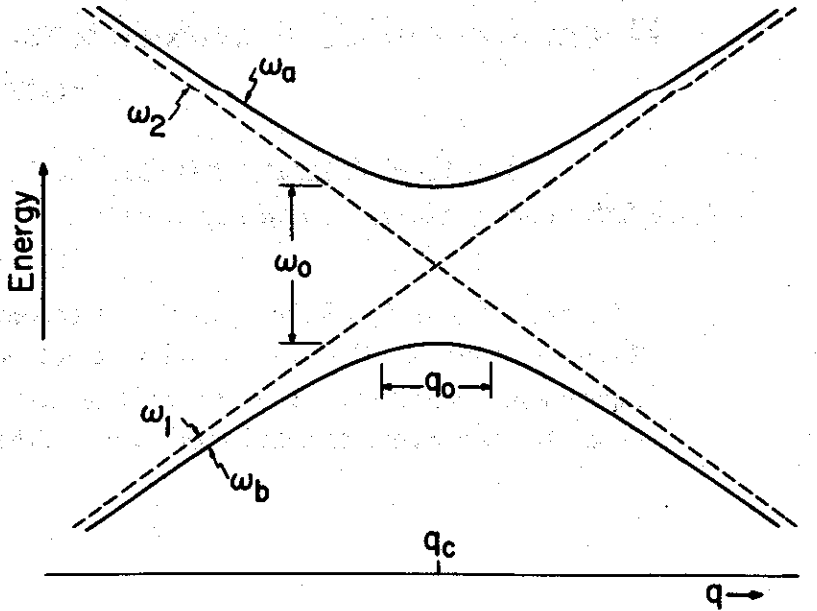
\includegraphics[width=.9\textwidth]{fig/Avoid_Crossing_With_Paramters.png}
    \end{figure}
    \end{minipage}
    \hfill
    \begin{minipage}{0.45\textwidth}
        Adyabatisite
        \begin{equation*}
            \Gamma = \eval{\frac{\omega^{2}_{0}}{4 \dv{r} \qty[\omega_{1}(r)-\omega_{2}(r)]}}_{r=r_{c}}
        \end{equation*}
        LZ geçiş olasılığı
        \begin{equation*}
            P = e^{-2\pi \Gamma}
        \end{equation*}
    \end{minipage}
\end{frame}

\begin{frame}
    \frametitle{$H_{\nu}+ H_{M}+ H_{EM}$ - Rezonanslar}
    Landau - Zener geçiş olasılığı, adyabatisiteye bağlıdır. Şartlar:
    \scriptsize
    \begin{enumerate}
        \item Hamiltonyen'in geçişten sorumlu olan elemanı konumdan bağımsız olmalıdır.
        \item Başlangıçtaki anlık (instantaneous) özdurumlar, başlangıç durumu ile aynı olmalıdır.
        \item Özdeğerlerin yakınlaştığı yani geçiş bölgesinde özdeğer farkları doğrusal olmalıdır.
    \end{enumerate}
    \normalsize

    \hrulefill
    
    Adyabatik evrim için 

    \begin{align*}
        \Gamma_{MSW} = \eval{\frac{\qty(\Delta s_{2\theta})^{2}}{4\dv{r}(\sqrt{2}G_{F}n_{b}(r)) }}_{r_{MSW}} \lesssim 1 \\
        \Gamma_{SFP} = \eval{\frac{(\mu B)^{2}}{\dv{r}(\sqrt{2}G_{F}(2Y_{e}-1)n_{b}(r))} }_{r_{SFP}}\lesssim 1
    \end{align*}

\end{frame}

\begin{frame}[noframenumbering,plain]
    \frametitle{İçerik}
    \begin{outline}
        \1[\checkmark] Giriş
        \1[\checkmark] Nötrino Salınım Kinematiği
        \1[\checkmark] Salınım Hamiltonyen'i ve Madde Etkileşimleri
        \2[\textendash] MSW Resonance
        \1[\checkmark] $H_{\nu}+ H_{M}+ H_{EM}$
        \2[\textendash] SFP Resonance
        \1[\textbullet] Analitik öngörüler
        \1[\textbullet] Simülasyonlar
        \1[\textbullet] Çekirdek Sentezlenmesi
    \end{outline}
\end{frame}


%\begin{frame}
%    \frametitle{Analitik Öngörüler}
%    Yoğunluk operatörü başlangıçta aşağıdaki gibi yazılır.
%    \begin{align*}
%        \hat{\rho}(R) = & \sum_{i,j} \mel{E_{i}(R)}{\hat{\rho}}{E_{j}(R)} \dyad{\Psi_{i}(R)}{\Psi_{j}(R)}\\
%                      = & \sum_{i,j} \rho_{ij}(R) \dyad{\Psi_{i}(R)}{\Psi_{j}(R)}
%    \end{align*}
%    Yoğunluk operatörü konuma bağlı evrilir.
%    \begin{equation*}
%        \hat{\rho}(r)= \sum_{a,b}\sum_{i,j}\qty(A_{ai}(r) \rho_{ij}(R) A^{\dagger}_{jb}(r)) C_{ij}(E)
%        \dyad{E_{i}(r)}{E_{j}(r)}
%    \end{equation*}
%    Burada $ C_{ij}(E)= \exp(-i\int^{r}_{R} \qty(E_{a}(x)- E_{b}(x)) \dd{x}) $.
%
%    $ A_{ij} $, özdurumların, $ \ket{E_{i}} $, birbirlerine geçiş genliğini veren matristir.
%\end{frame}

\begin{frame}
    \frametitle{Analitik Öngörüler - Adyabatik Evrim}
    Yoğunluk operatörünü, sonsuzdaki terim ve salınım olarak ikiye ayırabiliriz.
    \begin{align*}
        \hat{\rho}^{ad}(r) = & \hat{\bar{\rho}}^{ad}(\infty) + \hat{\rho}^{ad}_{sal}(r)\\
                      = &   \sum_{a}\sum_{i,j}\qty(A_{ai}(r) \rho_{ij}(R) A^{\dagger}_{ja}(r)) \dyad{E_{i}(r)}{E_{j}(r)} \\
                        & + \sum_{\substack{a,b\\ a \ne b}}\sum_{i,j}\qty(A_{ai}(r) \rho_{ij}(R) A^{\dagger}_{jb}(r)) C_{ij}(E) \dyad{E_{i}(r)}{E_{j}(r)}
    \end{align*}

    \begin{outline}
        \1[\textbullet] Salınımlar, decoherencedan dolayı çok uzakta yok olacaktır. 
        \1[\textbullet] {\color{red} Adyabatik evrim} için özdurumlar geçiş genliği {\color{red}$ A_{ij} $ matrisi birim matristir.}
        \1[\textbullet] Ortalama etrafında salınım, $ C_{ij}(E) $, salınım fazından kaynaklanır.
    \end{outline}

    \footnotesize
    \begin{equation*}
        C_{ij}(E) = \exp(-i\int^{R}_{r} \qty(E_{i}(x)- E_{j}(x)) \dd{x})
    \end{equation*}
    \normalsize
\end{frame}

\begin{frame}
    \frametitle{Analitik Öngörüler - Kısmen-Adyabatik Evrim}
    \begin{figure}[hbt!]
        \centering
        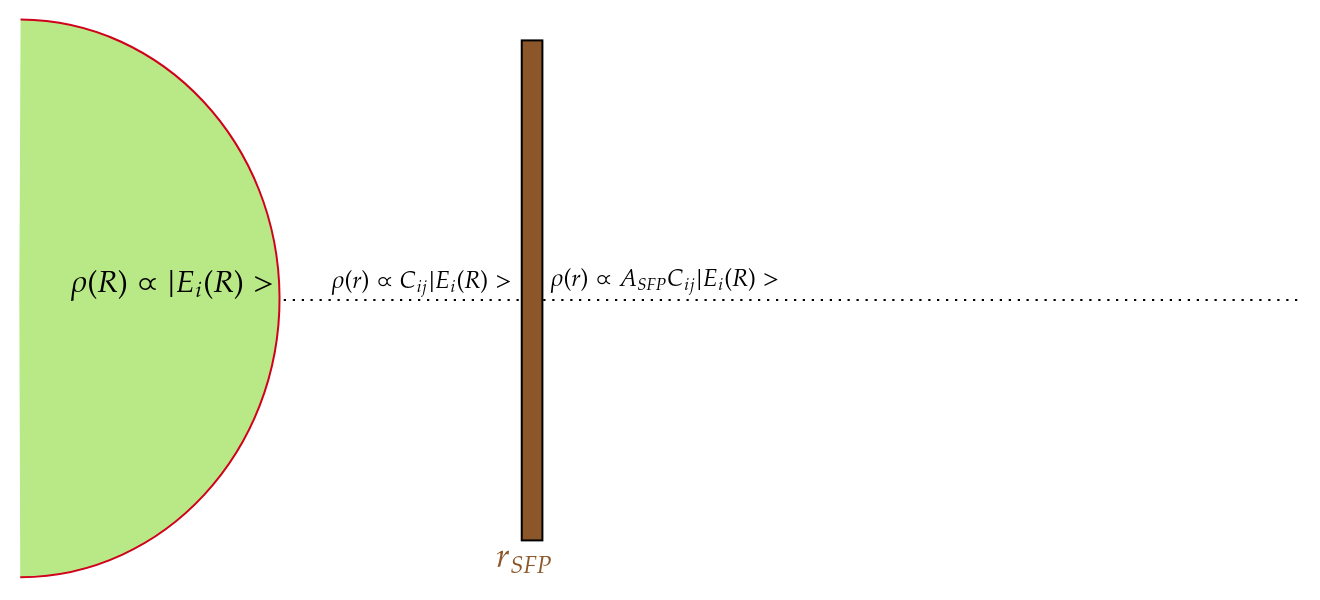
\includegraphics[width=\textwidth]{fig/rhoSFP.png}
    \end{figure}
\end{frame}

\begin{frame}
    \frametitle{Analitik Öngörüler - Kısmen-Adyabatik Evrim}
    \begin{figure}[hbt!]
        \centering
        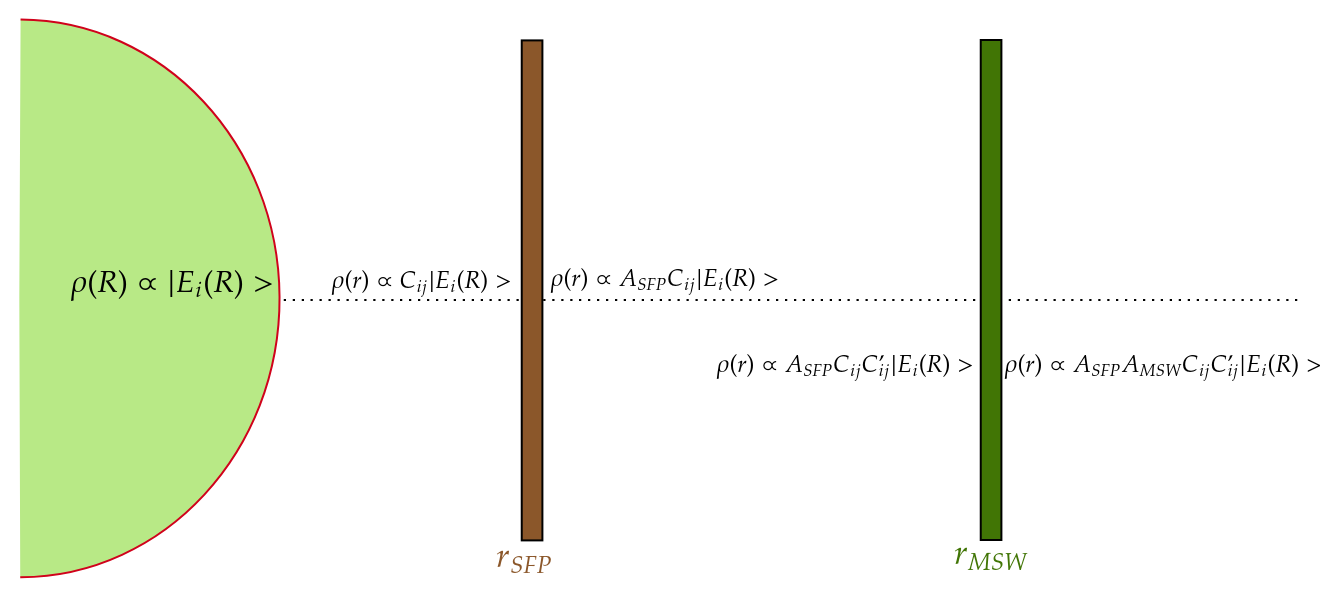
\includegraphics[width=\textwidth]{fig/rhoSFPMSW.png}
    \end{figure}
\end{frame}

\begin{frame}
    \frametitle{Analitik Öngörüler - Kısmen-Adyabatik Evrim}
    İki rezonans meydana geldiği kısmen-adyabatik evrimde, rezonansın meydana geldiği uzaklıklar arasındaki salınım fazı ve rezonans sırası önemlidir. Örneğin, ters hiyerarşi ve $ Y_{e}<0.5 $ için
    \begin{outline}
        \1[\textbf{1)}] $\rho_{ij}(R)C_{ij}(E) \rightarrow A^{\dagger}_{SFP}\rho_{ij}(R)C_{ij}(E)~A_{SFP}$
        \color{lightgray}
        \1[\textbf{2)}] $A^{\dagger}_{SFP}\rho_{ij}(R)C_{ij}(E)~A_{SFP} \rightarrow A^{\dagger}_{SFP} ~ \rho_{ij}(R)C_{ij}(E)~A_{SFP} C'_{ij}(E)$
        \1[\textbf{3)}] $A^{\dagger}_{SFP} ~ \rho_{ij}(R)C_{ij}(E)~A_{SFP} C'_{ij}(E)\rightarrow A^{\dagger}_{MSW}A^{\dagger}_{SFP}~\rho_{ij}(R)C_{ij}(E)~A_{SFP} C'_{ij}(E)~A_{MSW}$
    \end{outline}
    \color{lightgray}
    Geçiş matrisleri de aşağıdaki gibi tanımlıdır.
    \tiny
    \begin{align*}
        A =& A_{SFP} \times A_{MSW}\\
          =& \mqty(\sqrt{1-P_{SFP}} & -e^{-i\alpha}\sqrt{P_{SFP}} & 0 & 0 \\
      e^{i\alpha}\sqrt{P_{SFP}} & \sqrt{1-P_{SFP}} & 0 & 0 \\ 0 & 0 & 1 & 0 \\ 0 & 0 & 0 & 1) \times
      \mqty(1 & 0 & 0 & 0 \\ 0 & \sqrt{1-P_{MSW}} & -e^{-i\beta}\sqrt{P_{MSW}} & 0 \\ 0 & e^{i\beta}\sqrt{P_{MSW}} & \sqrt{1-P_{MSW}} & 0 \\ 0 & 0 & 0 & 1)
    \end{align*}
    \normalsize
\end{frame}

\begin{frame}[noframenumbering]
    \frametitle{Analitik Öngörüler - Kısmen-Adyabatik Evrim}
    İki rezonans meydana geldiği kısmen-adyabatik evrimde, rezonansın meydana geldiği uzaklıklar arasındaki salınım fazı ve rezonans sırası önemlidir. Örneğin, ters hiyerarşi ve $ Y_{e}<0.5 $ için
    \begin{outline}
        \1[\textbf{1)}] $\rho_{ij}(R)C_{ij}(E) \rightarrow A^{\dagger}_{SFP}\rho_{ij}(R)C_{ij}(E)~A_{SFP}$
        \1[\textbf{2)}] $A^{\dagger}_{SFP}\rho_{ij}(R)C_{ij}(E)~A_{SFP} \rightarrow A^{\dagger}_{SFP} ~ \rho_{ij}(R)C_{ij}(E)~A_{SFP} C'_{ij}(E)$
        \color{lightgray}
        \1[\textbf{3)}] $A^{\dagger}_{SFP} ~ \rho_{ij}(R)C_{ij}(E)~A_{SFP} C'_{ij}(E)\rightarrow A^{\dagger}_{MSW}A^{\dagger}_{SFP}~\rho_{ij}(R)C_{ij}(E)~A_{SFP} C'_{ij}(E)~A_{MSW}$
    \end{outline}
    \color{lightgray}
    Geçiş matrisleri de aşağıdaki gibi tanımlıdır.
    \tiny
    \begin{align*}
        A =& A_{SFP} \times A_{MSW}\\
          =& \mqty(\sqrt{1-P_{SFP}} & -e^{-i\alpha}\sqrt{P_{SFP}} & 0 & 0 \\
      e^{i\alpha}\sqrt{P_{SFP}} & \sqrt{1-P_{SFP}} & 0 & 0 \\ 0 & 0 & 1 & 0 \\ 0 & 0 & 0 & 1) \times
      \mqty(1 & 0 & 0 & 0 \\ 0 & \sqrt{1-P_{MSW}} & -e^{-i\beta}\sqrt{P_{MSW}} & 0 \\ 0 & e^{i\beta}\sqrt{P_{MSW}} & \sqrt{1-P_{MSW}} & 0 \\ 0 & 0 & 0 & 1)
    \end{align*}
    \normalsize
\end{frame}

\begin{frame}[noframenumbering]
    \frametitle{Analitik Öngörüler - Kısmen-Adyabatik Evrim}
    İki rezonans meydana geldiği kısmen-adyabatik evrimde, rezonansın meydana geldiği uzaklıklar arasındaki salınım fazı ve rezonans sırası önemlidir. Örneğin, ters hiyerarşi ve $ Y_{e}<0.5 $ için
    \begin{outline}
        \1[\textbf{1)}] $\rho_{ij}(R)C_{ij}(E) \rightarrow A^{\dagger}_{SFP}\rho_{ij}(R)C_{ij}(E)~A_{SFP}$
        \1[\textbf{2)}] $A^{\dagger}_{SFP}\rho_{ij}(R)C_{ij}(E)~A_{SFP} \rightarrow A^{\dagger}_{SFP} ~ \rho_{ij}(R)C_{ij}(E)~A_{SFP} C'_{ij}(E)$
        \1[\textbf{3)}] $A^{\dagger}_{SFP} ~ \rho_{ij}(R)C_{ij}(E)~A_{SFP} C'_{ij}(E)\rightarrow A^{\dagger}_{MSW}A^{\dagger}_{SFP}~\rho_{ij}(R)C_{ij}(E)~A_{SFP} C'_{ij}(E)~A_{MSW}$
    \end{outline}
    \color{lightgray}
    Geçiş matrisleri de aşağıdaki gibi tanımlıdır.
    \tiny
    \begin{align*}
        A =& A_{SFP} \times A_{MSW}\\
          =& \mqty(\sqrt{1-P_{SFP}} & -e^{-i\alpha}\sqrt{P_{SFP}} & 0 & 0 \\
      e^{i\alpha}\sqrt{P_{SFP}} & \sqrt{1-P_{SFP}} & 0 & 0 \\ 0 & 0 & 1 & 0 \\ 0 & 0 & 0 & 1) \times
      \mqty(1 & 0 & 0 & 0 \\ 0 & \sqrt{1-P_{MSW}} & -e^{-i\beta}\sqrt{P_{MSW}} & 0 \\ 0 & e^{i\beta}\sqrt{P_{MSW}} & \sqrt{1-P_{MSW}} & 0 \\ 0 & 0 & 0 & 1)
    \end{align*}
    \normalsize
\end{frame}

\begin{frame}[noframenumbering]
    \frametitle{Analitik Öngörüler - Kısmen-Adyabatik Evrim}
    İki rezonans meydana geldiği kısmen-adyabatik evrimde, rezonansın meydana geldiği uzaklıklar arasındaki salınım fazı ve rezonans sırası önemlidir. Örneğin, ters hiyerarşi ve $ Y_{e}<0.5 $ için
    \begin{outline}
        \1[\textbf{1)}] $\rho_{ij}(R)C_{ij}(E) \rightarrow A^{\dagger}_{SFP}\rho_{ij}(R)C_{ij}(E)~A_{SFP}$
        \1[\textbf{2)}] $A^{\dagger}_{SFP}\rho_{ij}(R)C_{ij}(E)~A_{SFP} \rightarrow A^{\dagger}_{SFP} ~ \rho_{ij}(R)C_{ij}(E)~A_{SFP} C'_{ij}(E)$
        \1[\textbf{3)}] $A^{\dagger}_{SFP} ~ \rho_{ij}(R)C_{ij}(E)~A_{SFP} C'_{ij}(E)\rightarrow A^{\dagger}_{MSW}A^{\dagger}_{SFP}~\rho_{ij}(R)C_{ij}(E)~A_{SFP} C'_{ij}(E)~A_{MSW}$
    \end{outline}
    Geçiş matrisleri de aşağıdaki gibi tanımlıdır.
    \tiny
    \begin{align*}
        A =& A_{SFP} \times A_{MSW}\\
          =& \mqty(\sqrt{1-P_{SFP}} & -e^{-i\alpha}\sqrt{P_{SFP}} & 0 & 0 \\
      e^{i\alpha}\sqrt{P_{SFP}} & \sqrt{1-P_{SFP}} & 0 & 0 \\ 0 & 0 & 1 & 0 \\ 0 & 0 & 0 & 1) \times
      \mqty(1 & 0 & 0 & 0 \\ 0 & \sqrt{1-P_{MSW}} & -e^{-i\beta}\sqrt{P_{MSW}} & 0 \\ 0 & e^{i\beta}\sqrt{P_{MSW}} & \sqrt{1-P_{MSW}} & 0 \\ 0 & 0 & 0 & 1)
    \end{align*}
    \normalsize
\end{frame}

\begin{frame}
    \frametitle{Analitik Öngörüler - Kısmen-Adyabatik Evrim}
    Kısmen-adyabatik evrim için yoğunluk operatörünü üçe ayırabiliriz.
    \begin{equation*}
        \hat{\overline{\rho}}(\infty) = \hat{\overline{\rho}}_{\text{ort}}(r) + \hat{\overline{\rho}}_{\text{hata}}(r) + {\color{gray}\hat{\overline{\rho}}_{\text{naKos}}(r)}
    \end{equation*}
    Ortalama terimi ve hata terimi $ \dyad{E_{i}}{E_{i}} $, köşegen olmayan terimler ise $ \dyad{E_{i}}{E_{j}} $, $ i \ne j $ terimlerinden oluşur.

    Ortalama teriminde $ \alpha,\beta $ Stokes fazları ve $C_{ij}$ ve $C'_{ij}$ salınım fazları yoktur.

\end{frame}

\begin{frame}
    \frametitle{Analitik Öngörüler - Kısmen-Adyabatik Evrim}
    \hrulefill
    \tiny

    \begin{equation*}
        \hat{\overline{\rho}}(\infty) = {\color{red}\hat{\overline{\rho}}_{\text{ort}}(r)} \pm \hat{\overline{\rho}}_{\text{hata}}(r)
    \end{equation*}
    \normalsize
    \hrulefill

    Ortalama terim
    \tiny
    \begin{align*}
        \hat{\overline{\rho}}_{\text{ort}}=& \bigg[(1-P_{SFP}) \rho_{11}(R)+ P_{SFP} \rho_{22}(R)\bigg] {\color{red}\dyad{E_{1}(r)}{E_{1}(r)}}\\
        &+ \bigg[\qty(1-P_{MSW})\qty(P_{SFP}\rho_{11}(R) +(1-P_{SFP})\rho_{22}(R))\\
        &~~~+ P_{MSW} \rho_{33}(R)\bigg] {\color{red}\dyad{E_{2}(r)}{E_{2}(r)}}\\
        &+ \bigg[P_{MSW}\qty(P_{SFP}\rho_{11}(R)+ (1-P_{SFP})\rho_{22}(R))\\
        &~~~+(1-P_{MSW})\rho_{33}(R)\bigg] {\color{red}\dyad{E_{3}(r)}{E_{3}(r)}}\\
    &+ \rho_{44}(R) {\color{red}\dyad{E_{4}(r)}{E_{4}(r)}}
    \end{align*}
    \normalsize
    \color{lightgray}
    Hata terimi
    \tiny
    \begin{align*}
        \hat{\overline{\rho}}_{\text{hata}}(r)=&2\bigg[\sqrt{(1-P_{SFP}) P_{SFP}}\rho_{12}(R)]\\
    &~~\times[(1-P_{MSW})\dyad{E_{2}(r)}{E_{2}(r)} -\dyad{E_{1}(r)}{E_{1}(r)}\bigg]\\
    &+ 2\bigg[\sqrt{(1-P_{MSW})P_{MSW}}\qty(\sqrt{P_{SFP}}\rho_{13}(R)+\sqrt{1-P_{SFP}}\rho_{23}(R))\bigg]\\ & ~~\qty[\dyad{E_{3}(r)}{E_{3}(r)} - \dyad{E_{2}(r)}{E_{2}(r)}]\\
    &+ 2 \bigg[P_{MSW}\sqrt{(1-P_{SFP}) P_{SFP}} \rho_{12}(R)\bigg]\dyad{E_{3}(r)}{E_{3}(r)}
    \end{align*}
    \normalsize
\end{frame}

\begin{frame}[noframenumbering]
    \frametitle{Analitik Öngörüler - Kısmen-Adyabatik Evrim}
    \hrulefill
    \tiny

    \begin{equation*}
        \hat{\overline{\rho}}(\infty) = \hat{\overline{\rho}}_{\text{ort}}(r) \pm {\color{red}\hat{\overline{\rho}}_{\text{hata}}(r)}
    \end{equation*}
    \normalsize
    \hrulefill
    
    \color{lightgray}
    Ortalama terim
    \tiny
    \begin{align*}
        \hat{\overline{\rho}}_{\text{ort}}=& \bigg[(1-P_{SFP}) \rho_{11}(R)+ P_{SFP} \rho_{22}(R)\bigg] \dyad{E_{1}(r)}{E_{1}(r)}\\
        &+ \bigg[\qty(1-P_{MSW})\qty(P_{SFP}\rho_{11}(R) +(1-P_{SFP})\rho_{22}(R))\\
        &~~~+ P_{MSW} \rho_{33}(R)\bigg] \dyad{E_{2}(r)}{E_{2}(r)}\\
        &+ \bigg[P_{MSW}\qty(P_{SFP}\rho_{11}(R)+ (1-P_{SFP})\rho_{22}(R))\\
        &~~~+(1-P_{MSW})\rho_{33}(R)\bigg] \dyad{E_{3}(r)}{E_{3}(r)}\\
    &+ \rho_{44}(R) \dyad{E_{4}(r)}{E_{4}(r)}
    \end{align*}
    \normalsize
    \color{black}
    Hata terimi
    \tiny
    \begin{align*}
        \hat{\overline{\rho}}_{\text{hata}}(r)=& 2\bigg[\sqrt{(1-P_{SFP}) P_{SFP}}\rho_{12}(R)]\\
    &~~\times[(1-P_{MSW}){\color{red}\dyad{E_{2}(r)}{E_{2}(r)}} -{\color{red}\dyad{E_{1}(r)}{E_{1}(r)}}\bigg]\\
    &+ 2\bigg[\sqrt{(1-P_{MSW})P_{MSW}}\qty(\sqrt{P_{SFP}}\rho_{13}(R)+\sqrt{1-P_{SFP}}\rho_{23}(R))\bigg]\\ & ~~\qty[{\color{red}\dyad{E_{3}(r)}{E_{3}(r)}} - {\color{red}\dyad{E_{2}(r)}{E_{2}(r)}}]\\
    &+ 2 \bigg[P_{MSW}\sqrt{(1-P_{SFP}) P_{SFP}} \rho_{12}(R)\bigg]{\color{red}\dyad{E_{3}(r)}{E_{3}(r)}}
    \end{align*}
    \normalsize
\end{frame}

\begin{frame}
    \frametitle{Simülasyonlar - ÇÇSN}
    \begin{minipage}{0.45\textwidth}
        \footnotesize
        \begin{outline}
            \1[\textbullet] Süpernova Evrelerinin Kısa Özeti
            \1[\textbullet] Çökme (Collapse)
            \1[\textbullet] Sekme (Bouncing)
            \1[\textbullet] Şok Dalgası Oluşumu
            \1[\textbullet] Nötrino Patlaması \\(Neutrino Burst)
            \1[\textbullet] Nötrino Isıtması  \\(Neutrino Heating)
        \end{outline}
        \begin{center}
            \textbf{“PATLAMA”}
        \end{center}
        \begin{outline}
            \1[\textbullet] {\color{red}“Soğuma”, $t= 1-10$ s (Cooling)}
        \end{outline}
        \normalsize
    \end{minipage}
    \hfill
    \begin{minipage}{0.45\textwidth}
        \begin{figure}[hbt!]
            \centering
            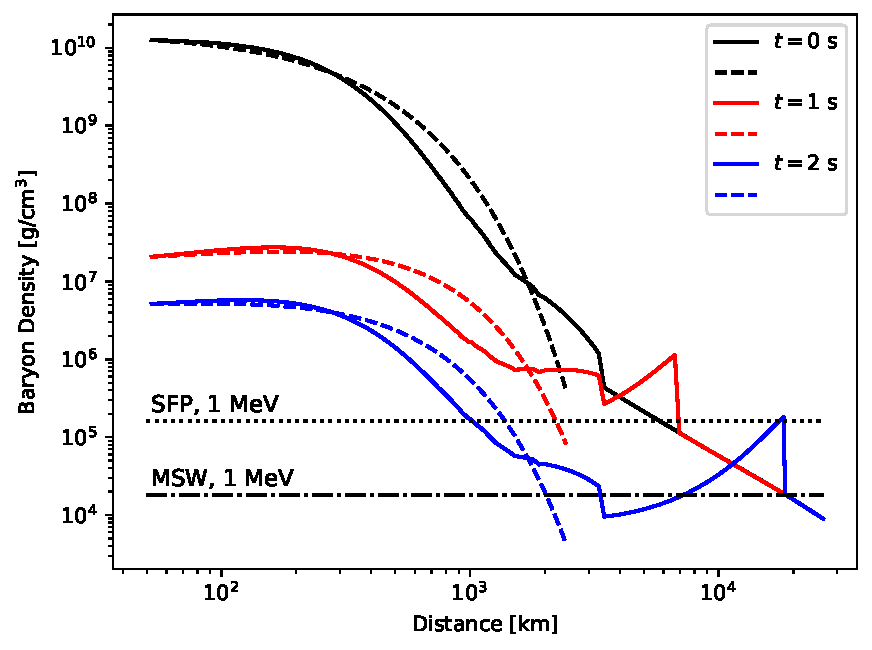
\includegraphics[width=1.1\textwidth]{fig/baryonDensity.pdf}
        \end{figure}
    \end{minipage}
\end{frame}

\begin{frame}
    \frametitle{Simülasyonlar - Başlangıç Koşulları}
    Oyuncak model için başlangıç koşulları
    \begin{figure}[hbt!]
        \centering
        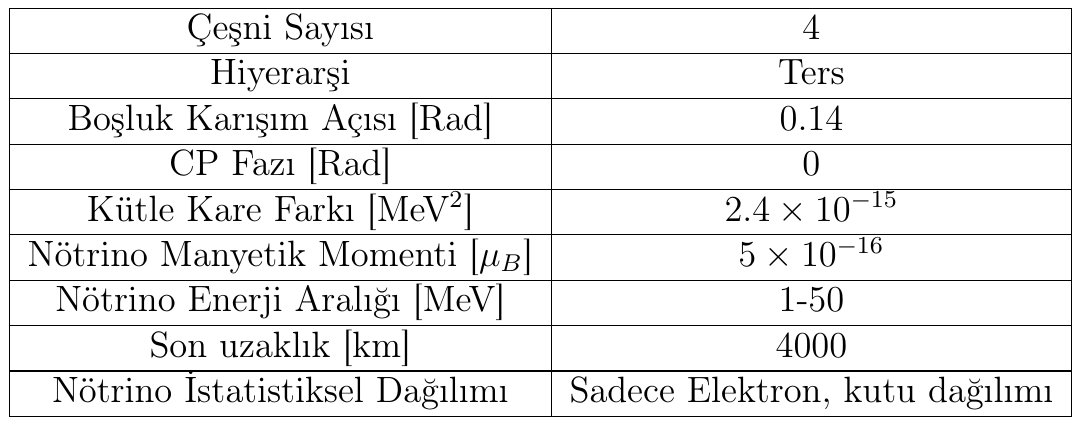
\includegraphics[width=.7\textwidth]{fig/baslangicKosullari.png}
    \end{figure}
    Fazları ortaya çıkarmak için ($B= 10^{15} (r_{Mag} \text{ [km]}/r)^{2}$ Gauss). Aşağıdaki değişkenler [km] birimindedir.
    \begin{figure}[hbt!]
        \centering
        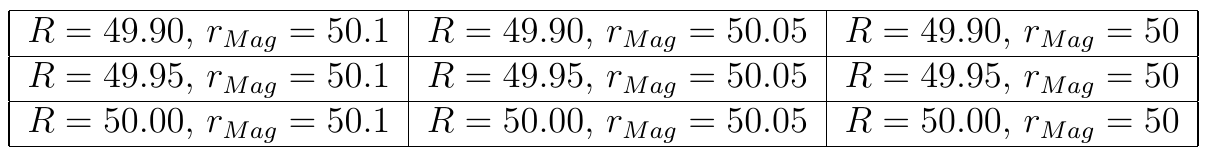
\includegraphics[width=\textwidth]{fig/baslangicKosullari9x9.png}
    \end{figure}
\end{frame}

\begin{frame}
    \frametitle{Simülasyonlar - theta0expNbB}
    \begin{figure}[hbt!]
        \centering
        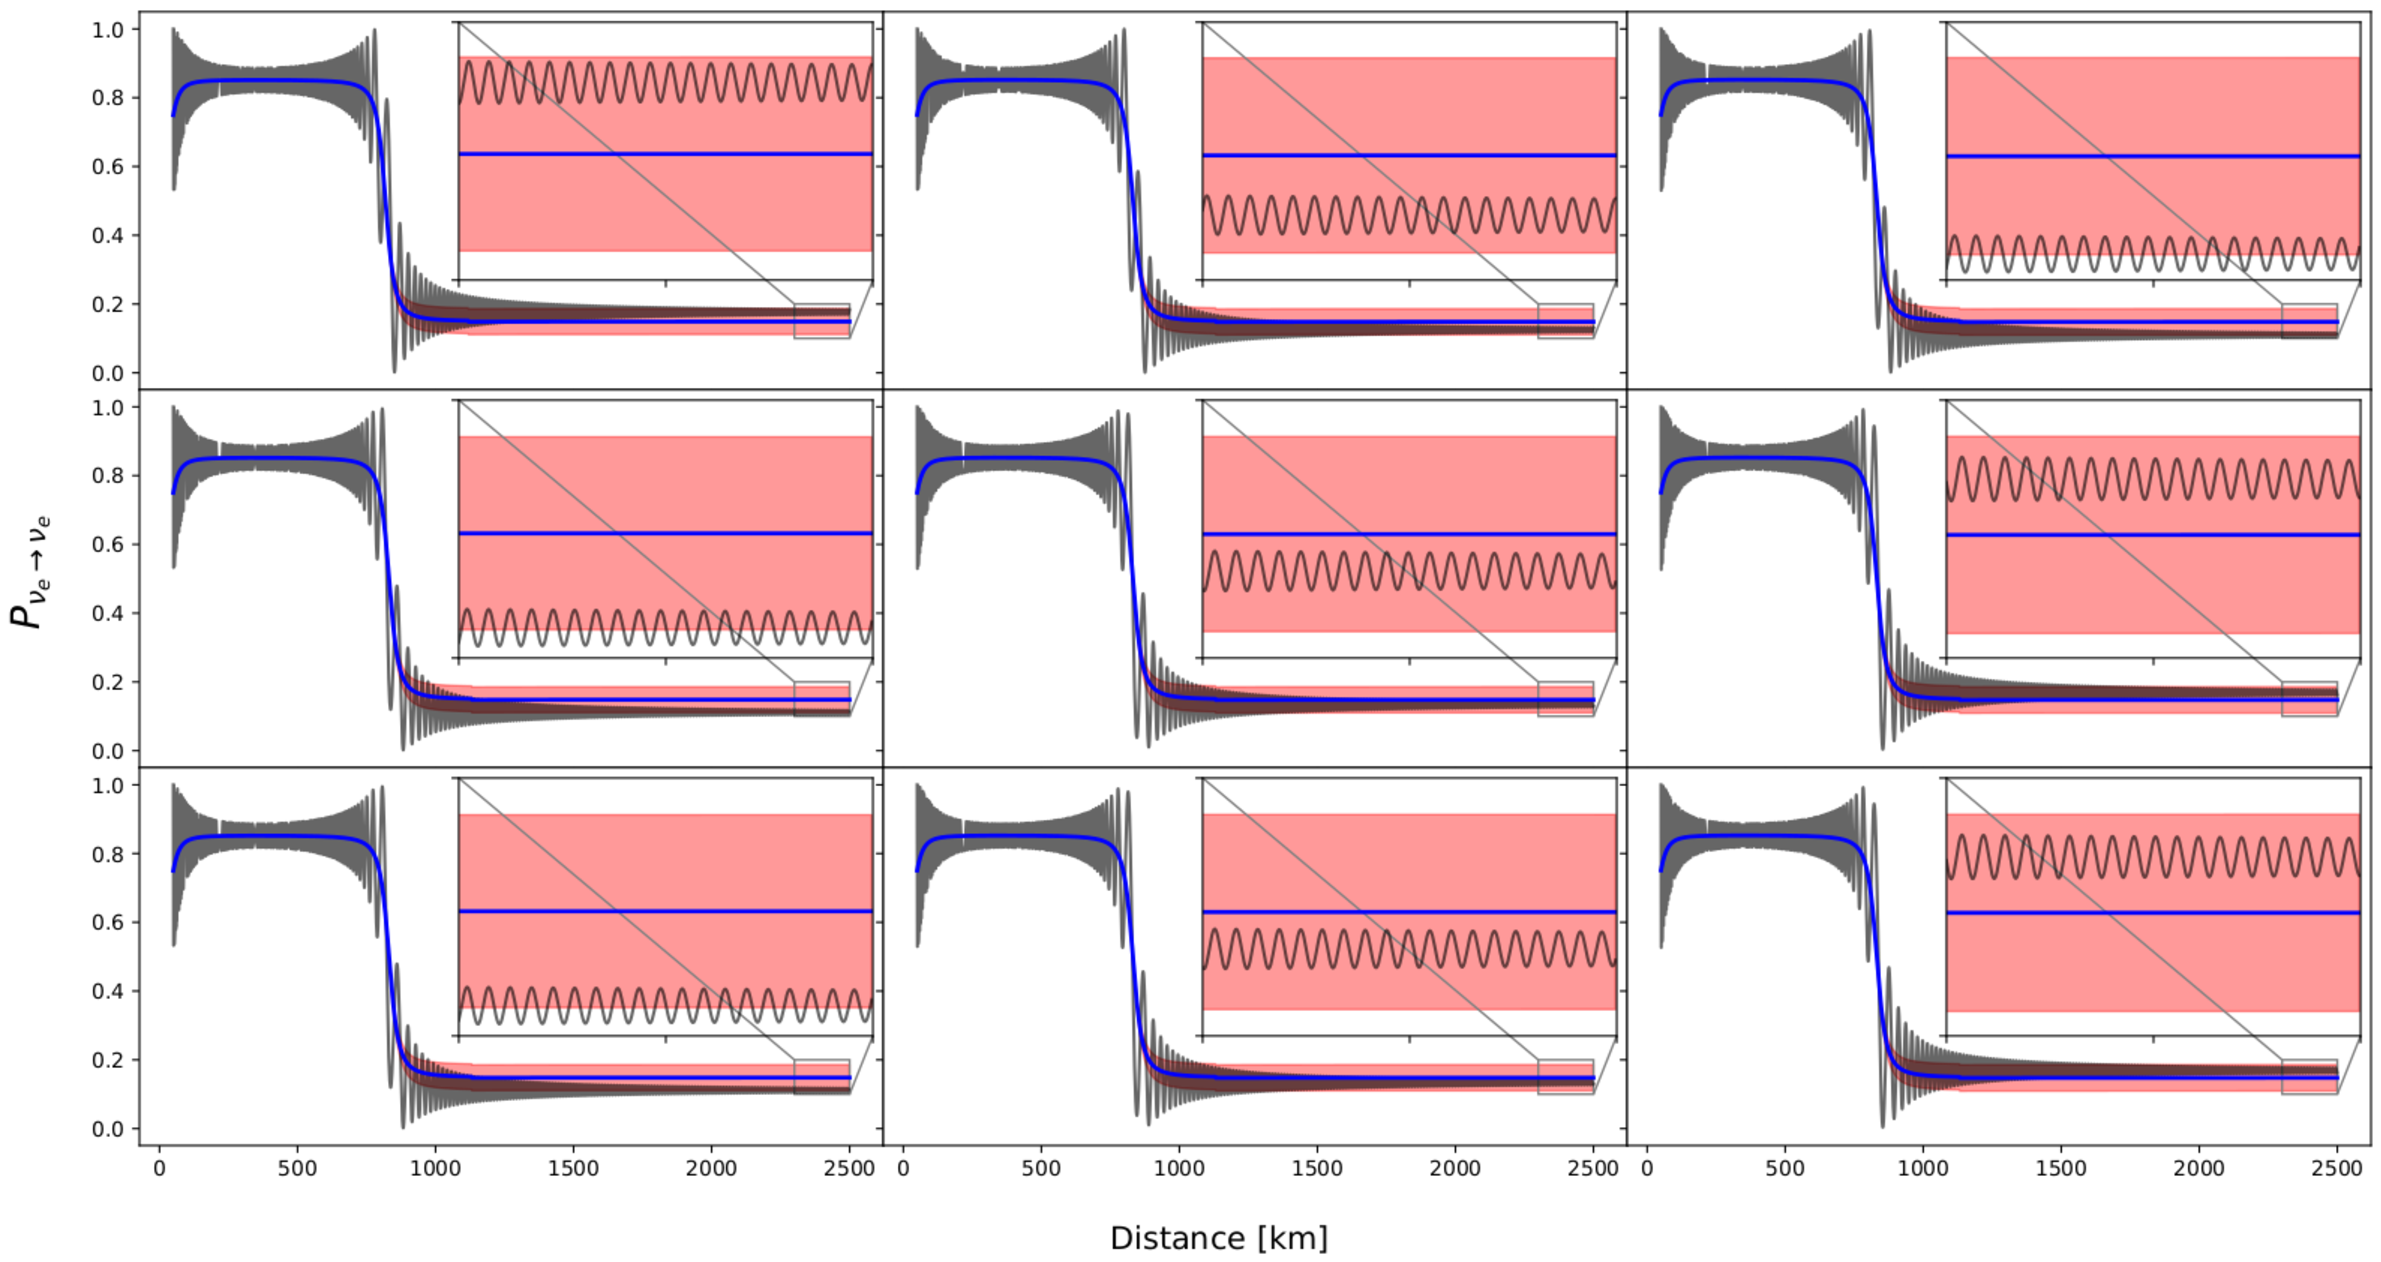
\includegraphics[width=\textwidth]{fig/P_ebeb2dist_initEbEb_10MeV_t3s_theta0.pdf}
    \end{figure}
\end{frame}

\begin{frame}
    \frametitle{Simülasyonlar - theta0expNbB}
    \hrulefill
    \tiny

    \begin{equation*}
        \hat{\overline{\rho}}(\infty) = {\color{blue}\hat{\overline{\rho}}_{\text{ort}}(r)} \pm {\color{red}\hat{\overline{\rho}}_{\text{hata}}(r)}
    \end{equation*}
    \normalsize
    \hrulefill
    \begin{figure}[hbt!]
        \centering
        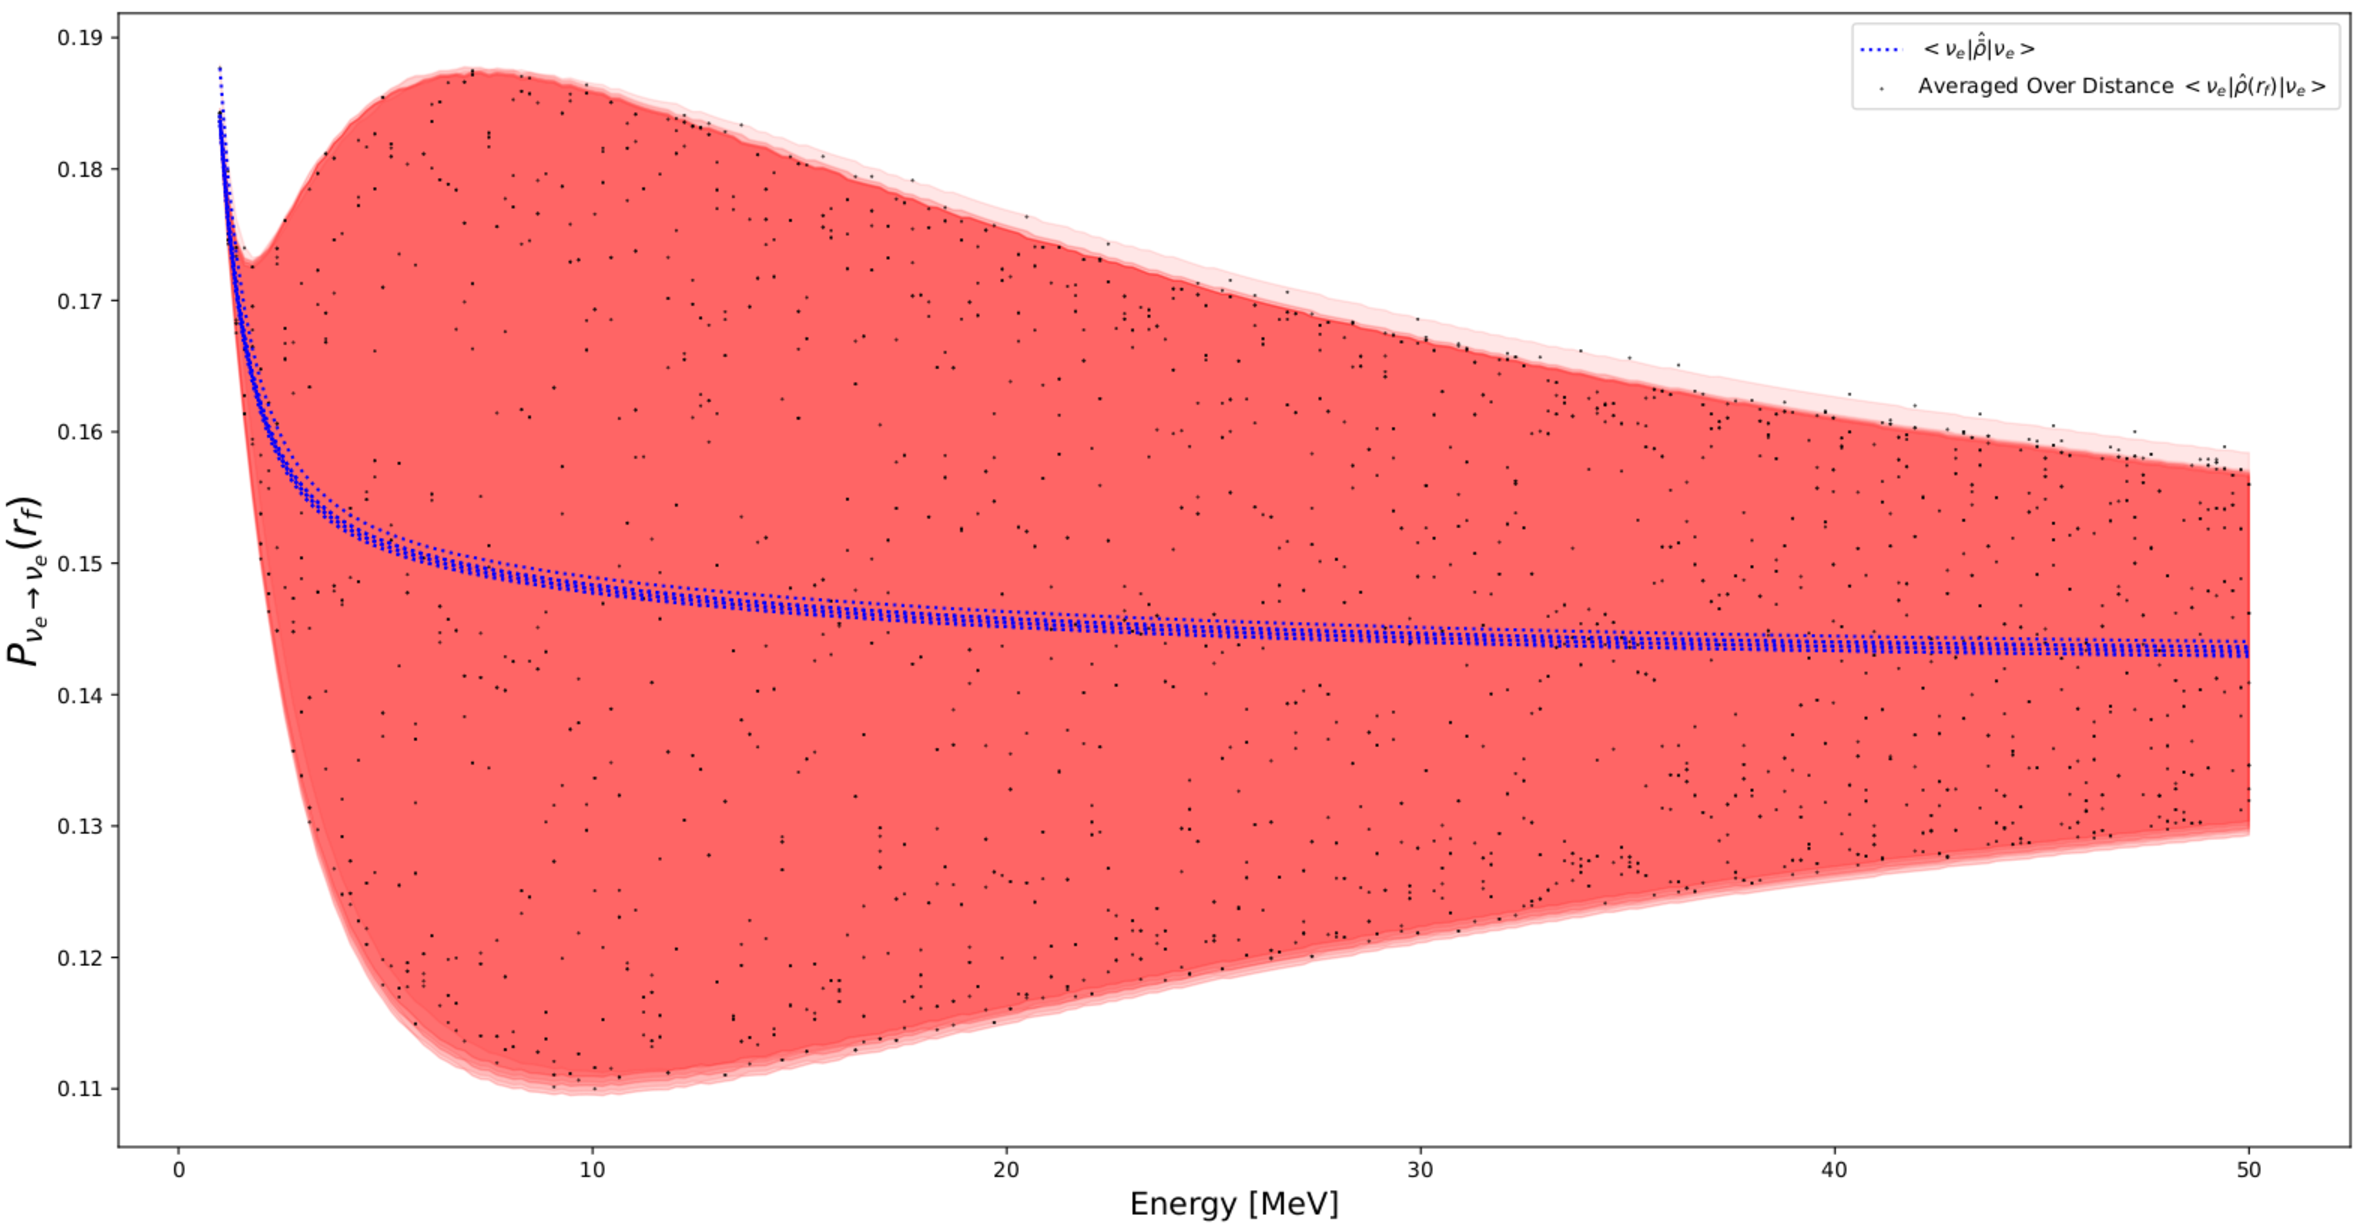
\includegraphics[width=\textwidth]{fig/theta0expNbB_energySpec_theta0_averaged.pdf}
    \end{figure}
\end{frame}

\begin{frame}
    \frametitle{Simülasyonlar - theta014expNbB, $t=5$ s}
    \begin{figure}[hbt!]
        \centering
        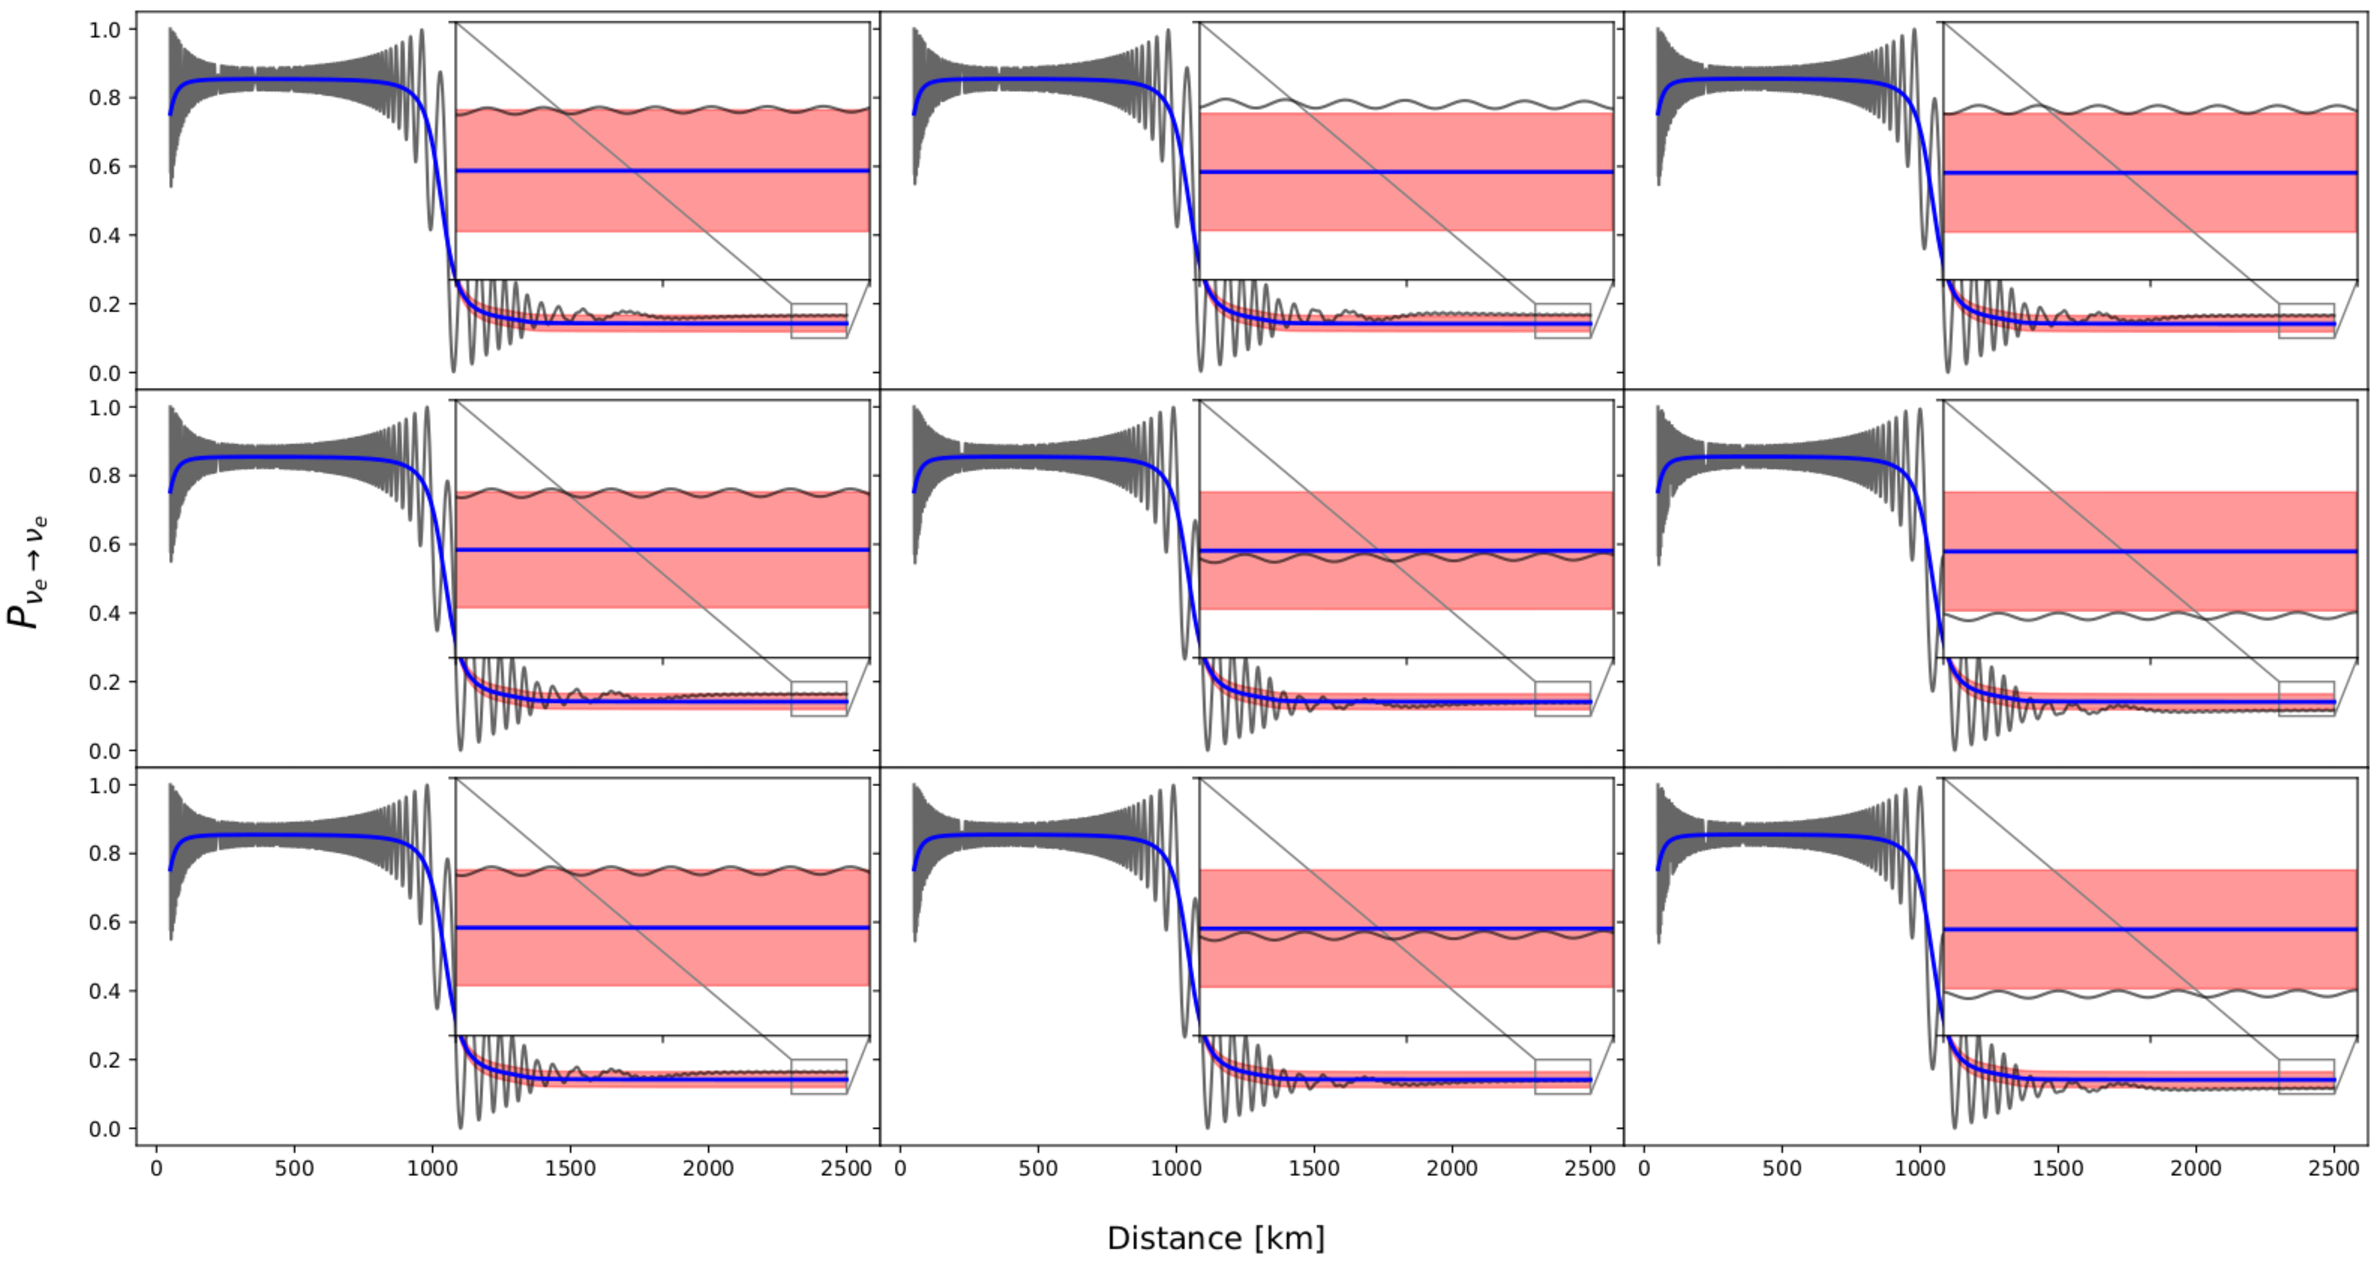
\includegraphics[width=\textwidth]{fig/theta014expNbB_9x9_10MeV.pdf}
    \end{figure}
\end{frame}

\begin{frame}
    \frametitle{Simülasyonlar - theta014expNbB, $t=5$ s}
    Boşluk karışım açısı sıfırdan farklı olduğunda hem SFP hem de MSW rezonansları meydana gelir.
    \begin{align*}
        \Delta r_{MSW}/2 =& \frac{-r_{mat}}{2} \ln(\frac{c_{2\theta} - s_{2\theta}}{c_{2\theta} + s_{2\theta}}) \\
        \Delta r_{SFP}/2 =& \frac{-r_{mat}}{2} \ln(\frac{\Delta c_{2\theta}-\mu B_{1}}{\Delta c_{2\theta}+\mu B_{1}}) \\
        \eval{\frac{\abs{r^{SFP} - r^{MSW}}}{r^{SFP}_{hw}+r^{MSW}_{hw}}}_{t=1,3,5 \text{ s}} =& 3.31\text{, } 2.60\text{, } 2.24
    \end{align*}
\end{frame}

\begin{frame}[noframenumbering]
    \frametitle{Simülasyonlar - theta014expNbB, $t=1,3,5$ s}
    Baryon yoğunluğu azaldığında SFP ve MSW rezonansları yakınlaşır.
    \begin{figure}[hbt!]
        \centering
        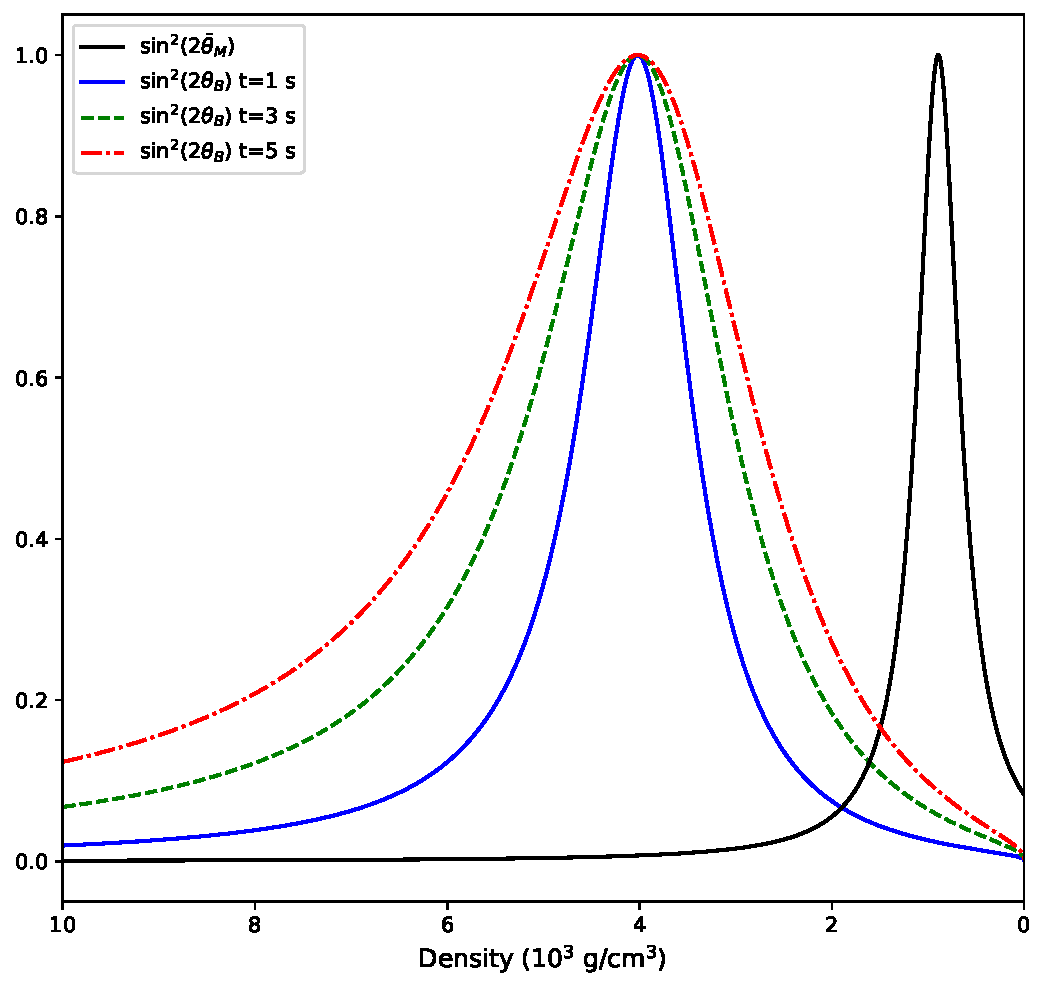
\includegraphics[width=.7\textwidth]{fig/widthCompare3_nbInverted_40MeV_IH_t135s_sqr_croped.pdf}
    \end{figure}
\end{frame}

\begin{frame}
    \frametitle{Simülasyonlar - theta014expNbB, $t=1$ s}
    \hrulefill
    \tiny
    
    NH: $\nu_{\bar{e}} \rightarrow \nu_{x} \rightarrow \nu_{e} $, \qquad IH: $\nu_{e} \rightarrow \nu_{\bar{x}} \rightarrow \nu_{\bar{e}} $\\
    \hrulefill
    \normalsize
    \begin{figure}[hbt!]
        \centering
        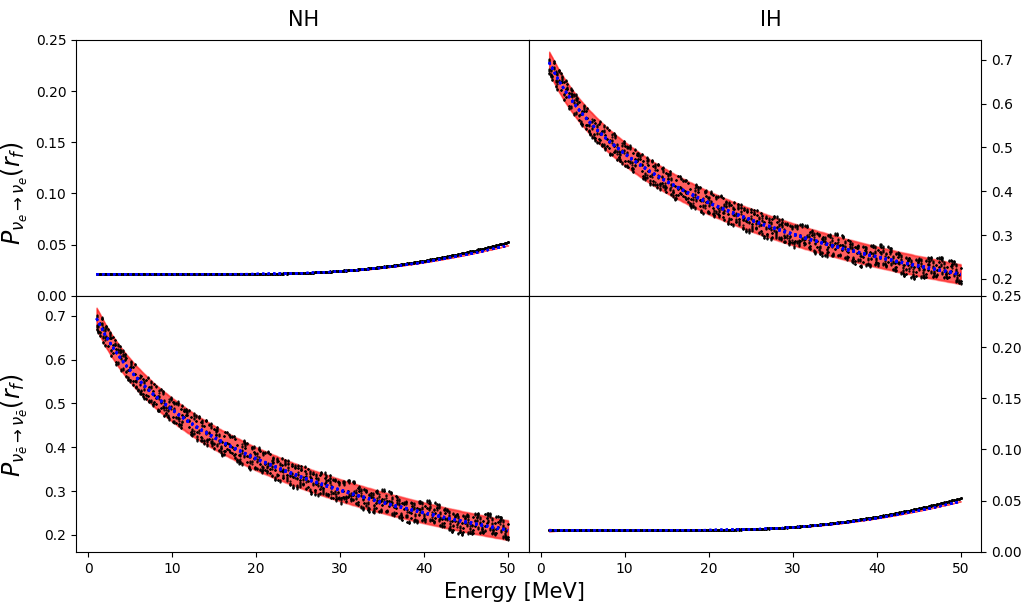
\includegraphics[width=\textwidth]{fig/theta014expNbB_t1s_energySpec_theta0_averaged.png}
    \end{figure}
\end{frame}

\begin{frame}
    \frametitle{Simülasyonlar - theta014expNbB, $t=3$ s}
    \begin{figure}[hbt!]
        \centering
        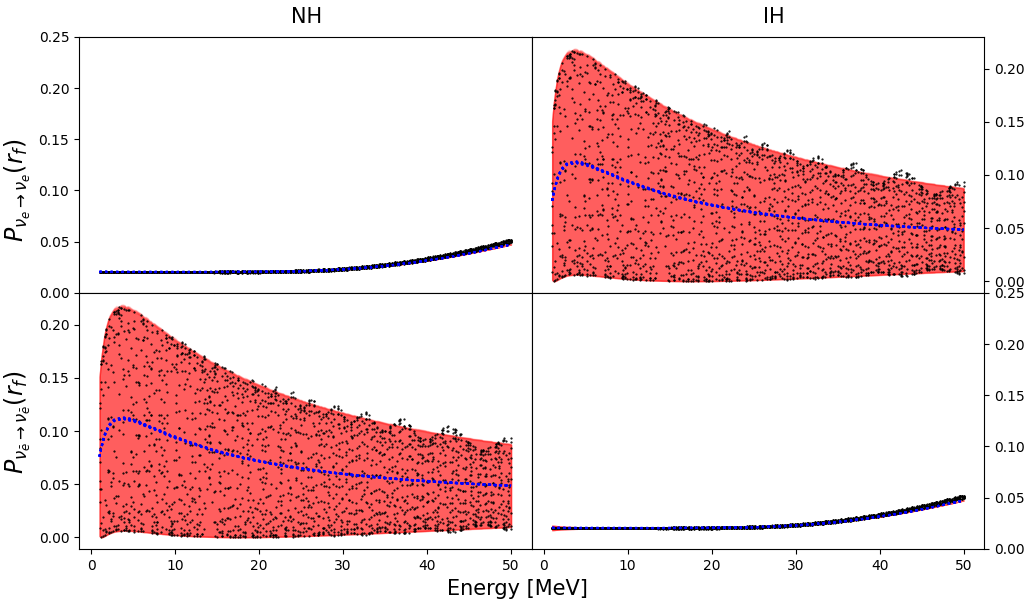
\includegraphics[width=\textwidth]{fig/theta014expNbB_t3s_energySpec_theta0_averaged.png}
    \end{figure}
\end{frame}

\begin{frame}
    \frametitle{Simülasyonlar - theta014expNbB, $t=5$ s}
    \begin{figure}[hbt!]
        \centering
        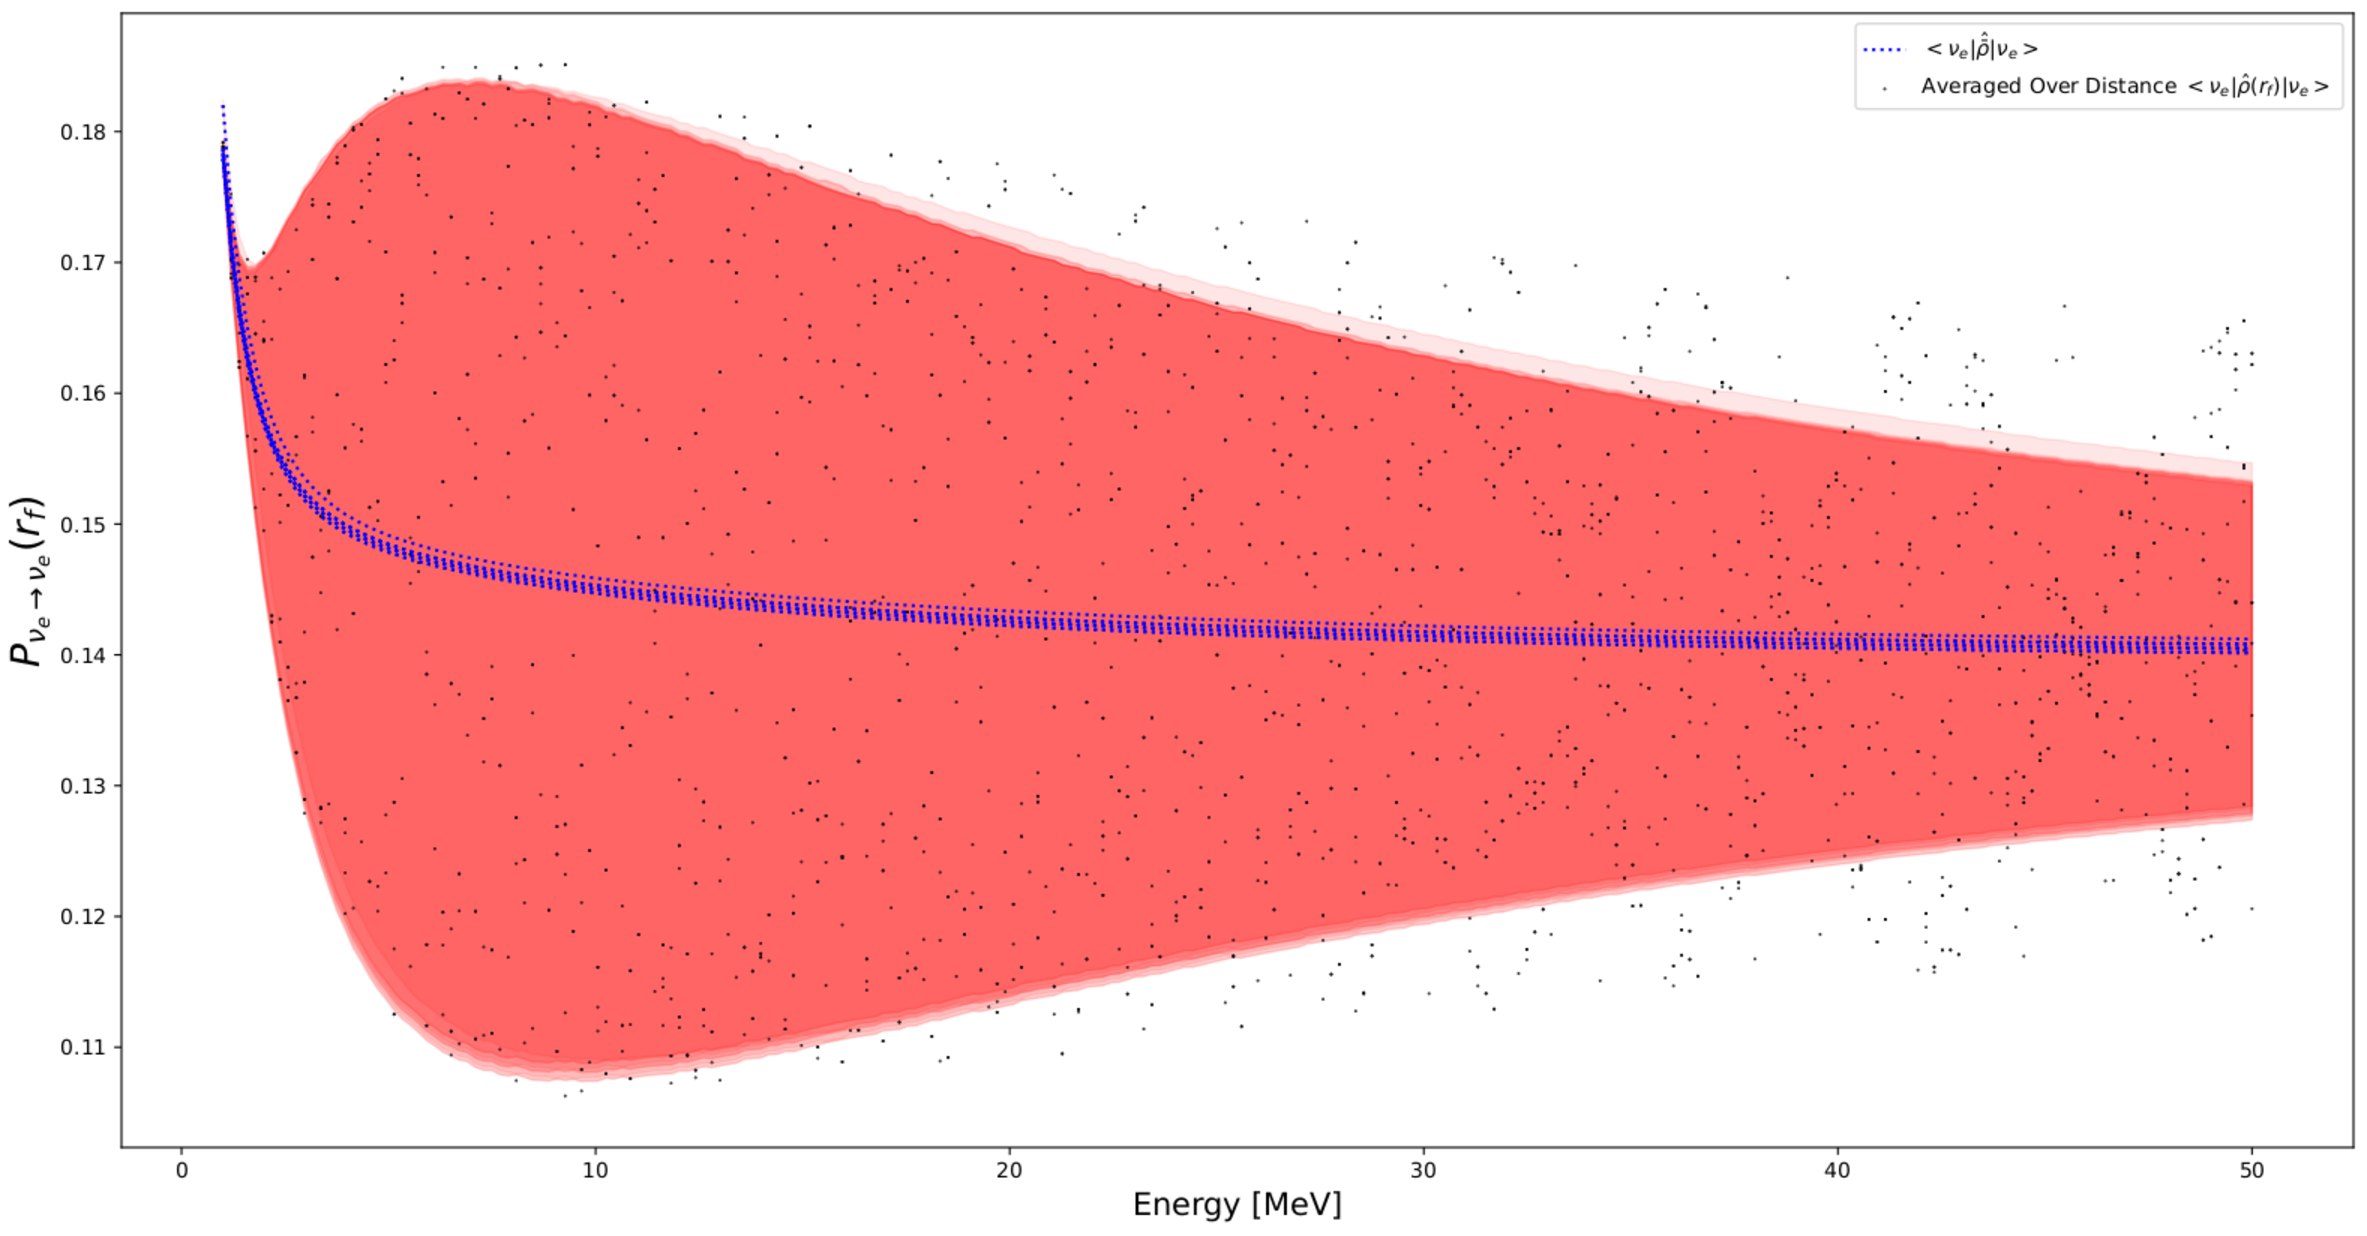
\includegraphics[width=\textwidth]{fig/theta014expNbB_energySpec_theta0_averaged.pdf}
    \end{figure}
\end{frame}

\begin{frame}
    \frametitle{Simülasyonlar - Fermi-Dirac Dağılımı, $t=1,2,3$ s}
    \begin{figure}[hbt!]
        \centering
        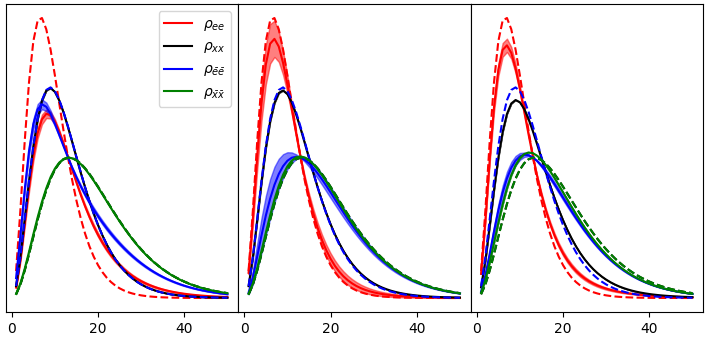
\includegraphics[width=\textwidth]{fig/yatayFermiSpec_t135.png}
    \end{figure}
\end{frame}

\begin{frame}
    \frametitle{Simülasyonlar - t5sCollnuNoB}
    \begin{figure}[hbt!]
        \centering
        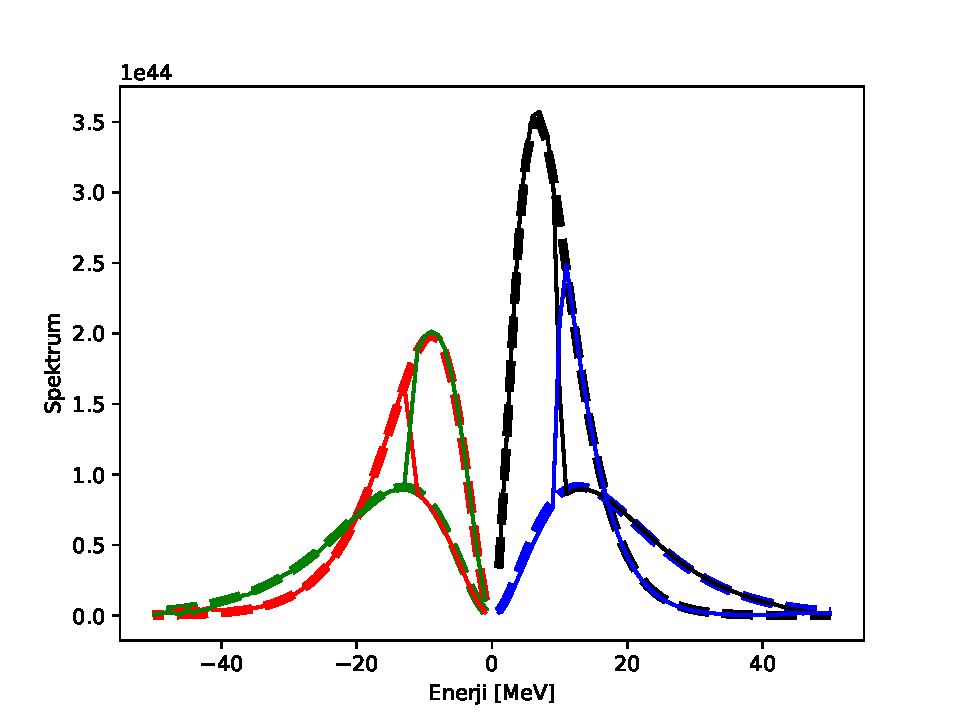
\includegraphics[width=\textwidth]{fig/t5sCollnuNoB_spectrum.pdf}
    \end{figure}
\end{frame}
\begin{frame}
    \frametitle{Simülasyonlar - t5sCollnuB}
    \begin{figure}[hbt!]
        \centering
        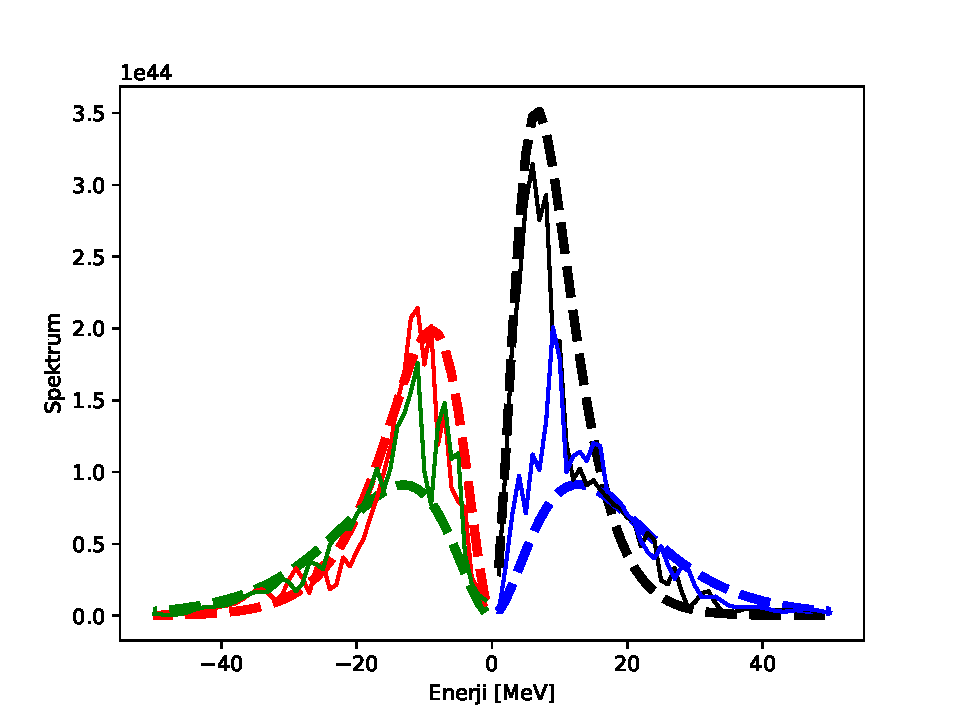
\includegraphics[width=\textwidth]{fig/t5sCollnuB_spectrum.pdf}
    \end{figure}
\end{frame}

\begin{frame}
    \frametitle{Çekirdek Sentezlenmesi}
    \begin{minipage}{0.45\textwidth}
        \begin{figure}[hbt!]
            \centering
            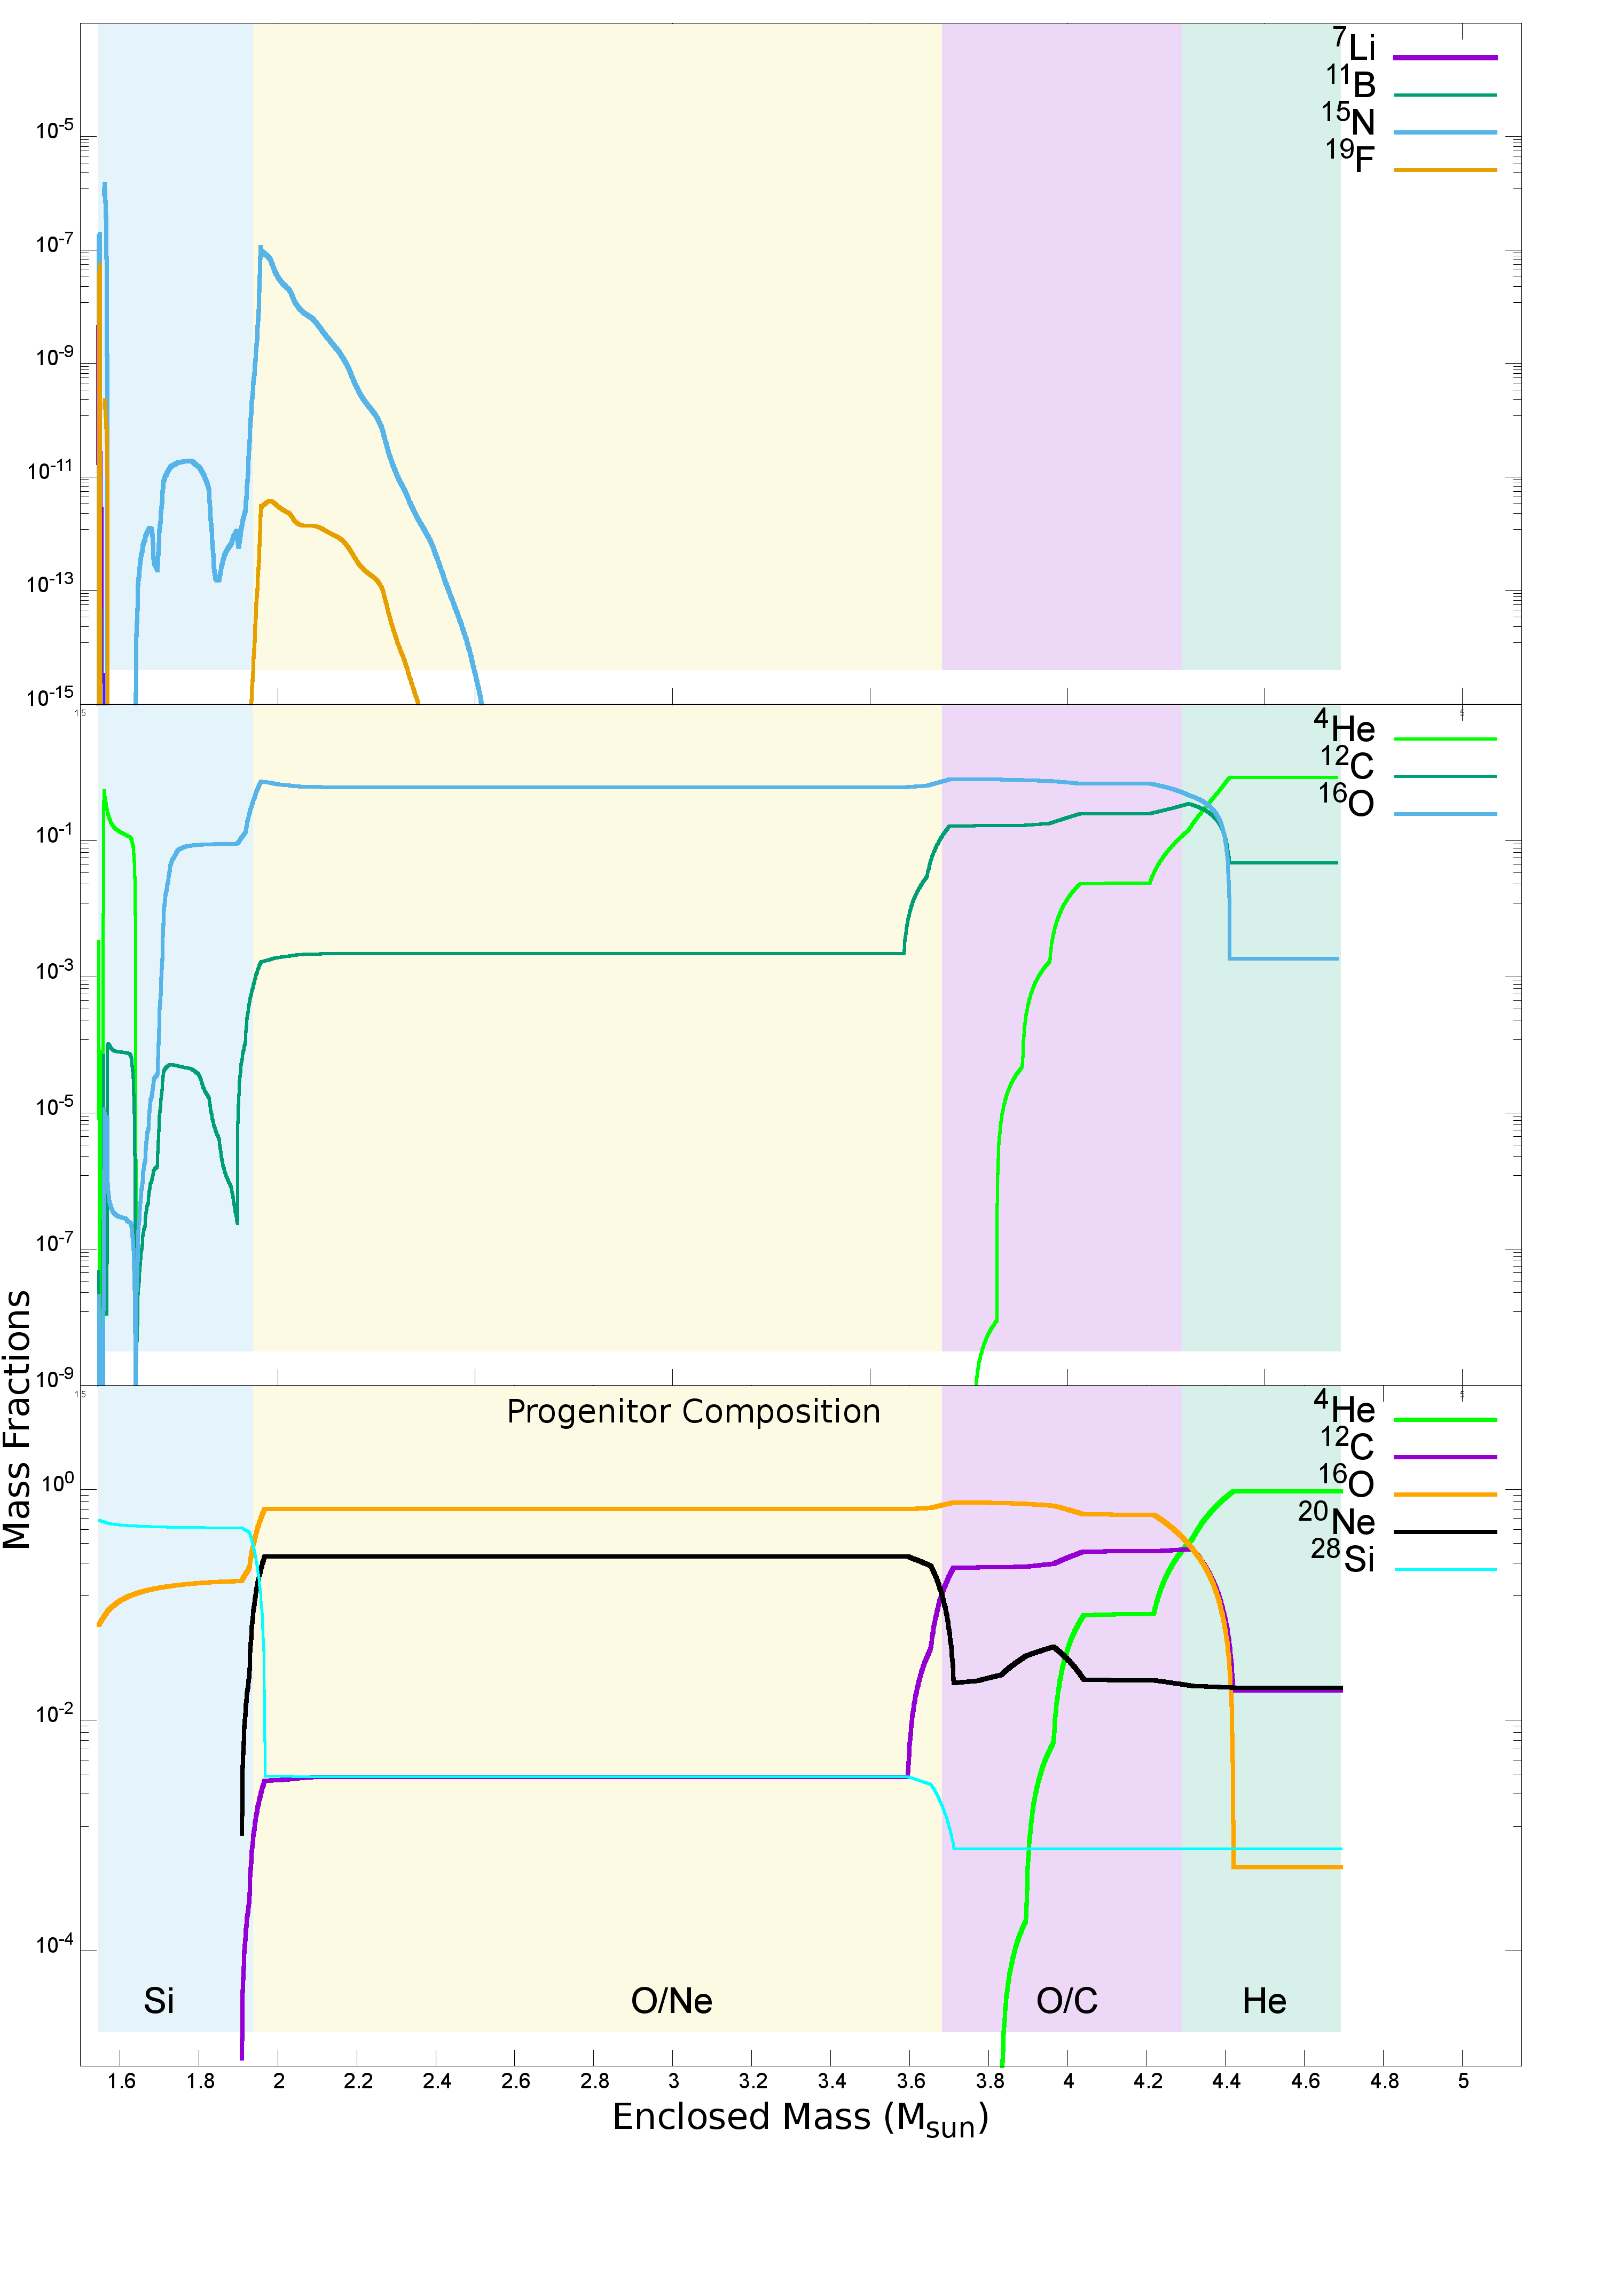
\includegraphics[width=\textwidth]{fig/abundadecay_noNu_he4li7b11c12n15o16f19_hor.png}
        \end{figure}
    \end{minipage}
    \hfill
    \begin{minipage}{0.45\textwidth}
        \begin{figure}[hbt!]
            \centering
            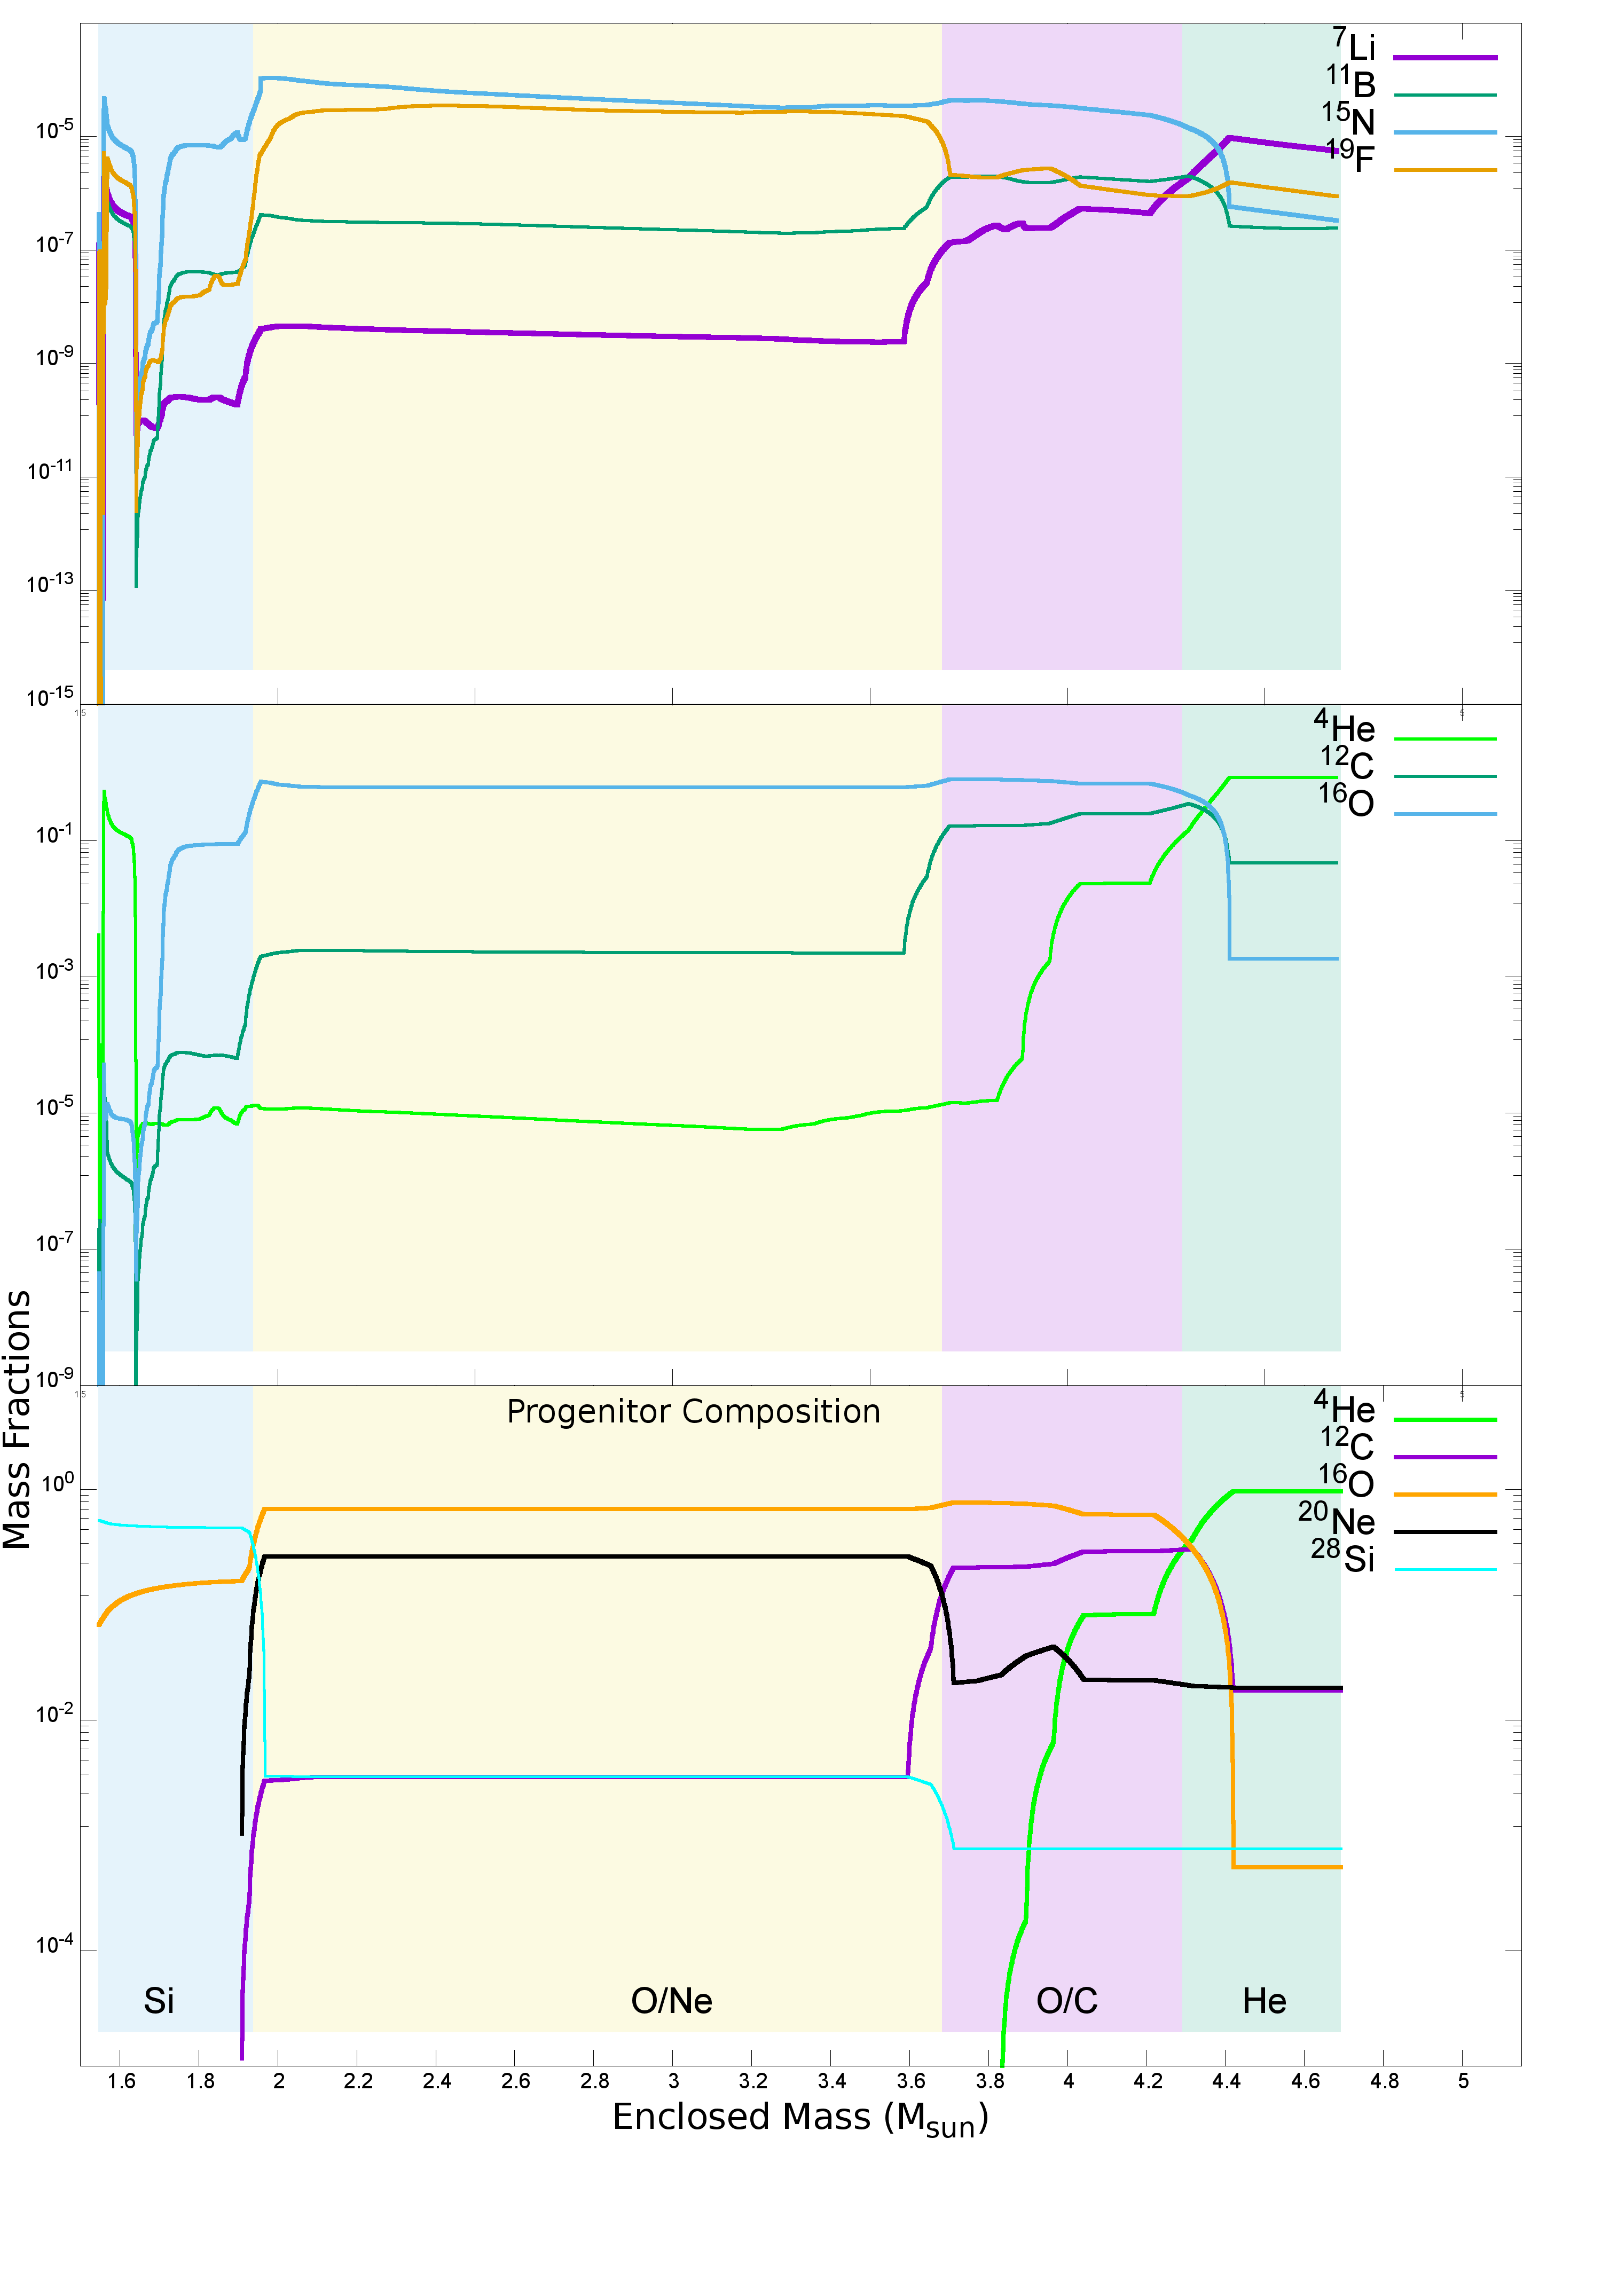
\includegraphics[width=\textwidth]{fig/abundadecay_he4li7b11c12n15o16f19_hor.png}
        \end{figure}
    \end{minipage}
\end{frame}

\begin{frame}
    \frametitle{Çekirdek Sentezlenmesi}
    \begin{figure}[hbt!]
        \centering
        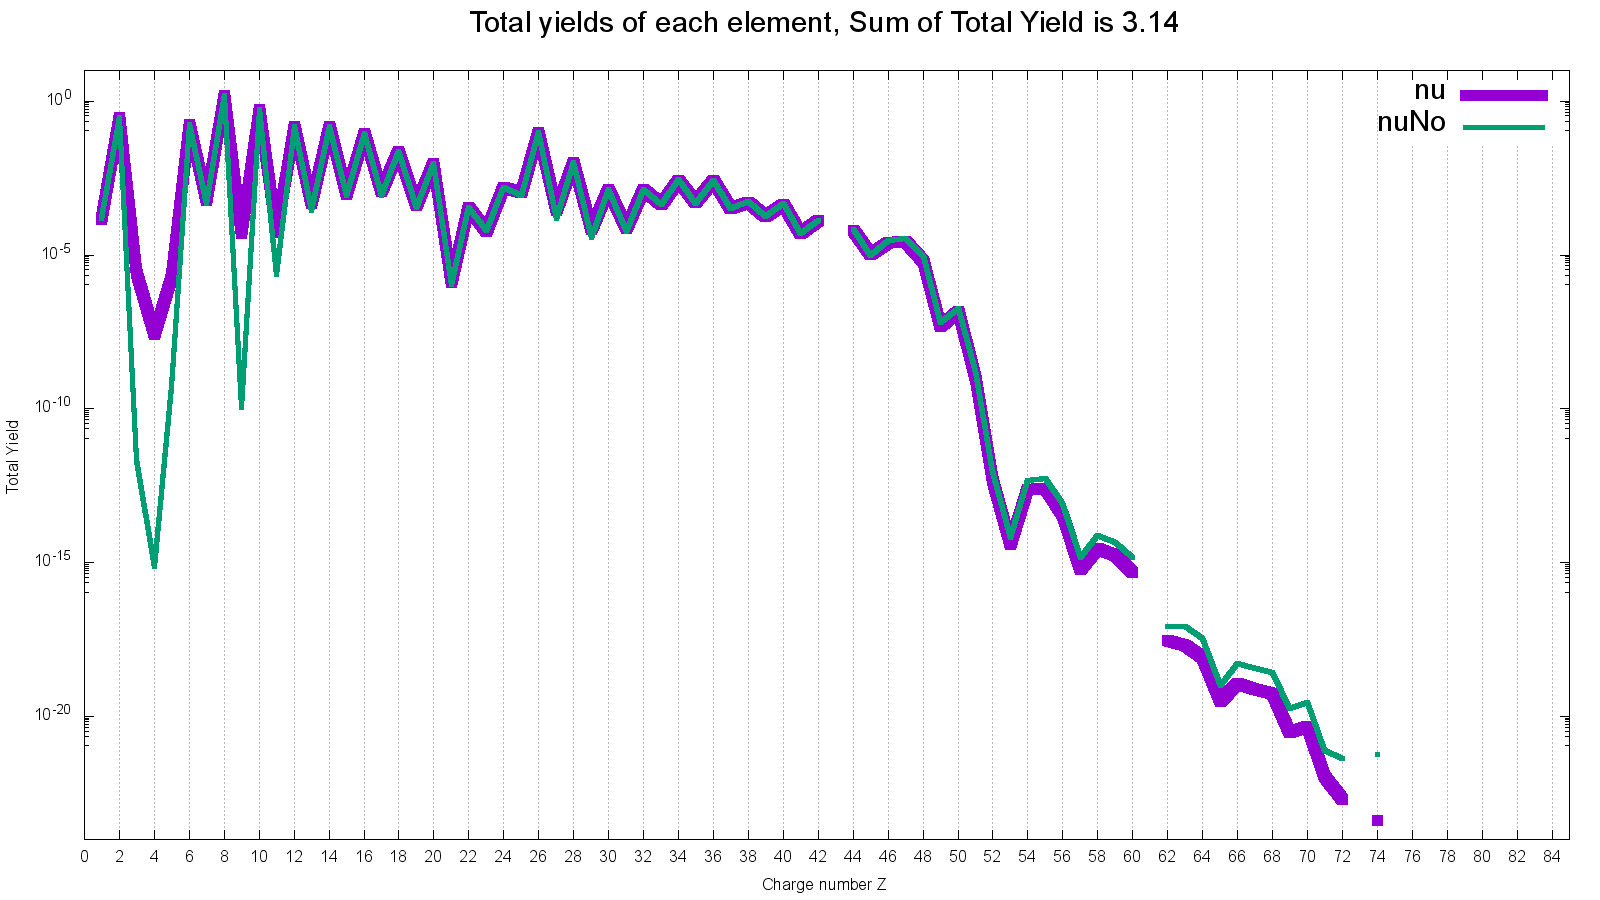
\includegraphics[width=\textwidth]{fig/abundadecay_Z_TotalYields_nu_nuNo.png}
    \end{figure}
\end{frame}

\begin{frame}
    \frametitle{Sonuçlar}
    \scriptsize
    \begin{outline}
        \1[\textbullet] Düşük manyetik alan için {\color{red}tedirgenmiş çözümler} elde ettik.
        \1[\textbullet] {\color{red}Eksponansiyel azalan baryon profili ve sabit manyetik alan için analitik çözümlerin} Kummer fonksiyonları cinsinden yazılabildiğini bulduk.
        \1[\textbullet] Adyabatik olmayan çeşni evriminde yoğunluk matrisinin analitik ifadesini elde ettik. Stokes fazını ve donmuş fazı hata olarak adlandırıp ortalama sonuçlara ekledik.
        \1[\textbullet] {\color{red}Analitik sonuçlar ile sayısal sonuçları karşılaştırdık.} Sonuçlarımız sıfır {\color{red}boşluk karışım açısı ve $ t=1,2,3 $ s} profilleri için tutarlı olduğunu gördük.
        \1[\textbullet] {\color{red}$ t=4,5 $ s profilleri için üç çeşni etkileri} ortaya çıkmaktadır. Üç çeşni etkileri SFP ve MSW rezonansların birbirine yakınlaşmasından kaynaklandığını bulduk ve yakınlık derecesini niceliksel olarak belirledik.
        \1[\textbullet] Nötrino öz-kırılımının etkisine baktık ve manyetik alan etkileşimlerinin elektron antinötrinosunun sıcaklığını arttırdığını bulduk.
        \1[\textbullet] Nötrino sentezlenmesinin Lityum$ ^{7} $ ve Bor$ ^{11} $ izotoplarının sentezlenmesinde büyük önem taşımaktadır.
    \end{outline}
    
    Bir sonraki adımda 
    \begin{outline}
        \1[\textbullet] SFP ile MSW rezonansı arasında kalan donmuş fazların çeşni evrimine olan katkısı incelenecektir.
        \1[\textbullet] Elektron kesrinin ani değişiminden kaynaklanan süreksizlikler ve çeşni evrimine olan etkisine bakılacaktır.
    \end{outline}
    \normalsize
    
\end{frame}

\begin{frame}[plain,noframenumbering]
    \huge
    \begin{center}
        Teşekkür ederim.
    \end{center}
\end{frame}

\begin{frame}[plain, noframenumbering]
    \frametitle{Referanslar}
    \footnotesize
    \begin{itemize}
        \item[] [Raffelt, 1996] G. G. Raffelt, Stars as laboratories for fundamental physics: The astrophysics of neutrinos, axions, and other weakly interacting particles. University of Chicago press, 1996.        
        \item[] [Giunti, 2007] C. Giunti and C. W. Kim, Fundamentals of Neutrino Physics and Astrophysics. Oxford University Press, 2007.        
        \item[] [Rubbmark, 1981]  J. R. Rubbmark, M. M. Kash, M. G. Littman, and D. Kleppner, “Dynamical effects at avoided level crossings: A study of the Landau-Zener effect using Rydberg atoms,” Physical Review A, vol. 23, pp. 3107-3117, June 1981.
    \end{itemize}
    \normalsize
\end{frame}



\end{document}